  
\section{Data Analysis}
\label{sec:data-analysis}

%The TIM Hamiltonian for calculating the occupation number versus Trotter step served as a quantum computing application example for studying the stability and reproducibility of these computations on the Boeblingen platform.  

In this section, we will focus on analyzing the results from a direct calculation of the TIM occupation index and from a detailed study of 2 different sets of CNOT gate configurations (circuit 1 and circuit 2) derived from the CNOT gate sequences in the TIM Hamiltonian using cycle benchmarking. Measurements were done with the occupation index and for cycle benchmarking of circuits 1 and 2 at specific time periods within the same day, at the same set of specific time periods for different days, and also with the placement of these two circuits on groups of 4 qubits located in different physically distinct areas on the Boeblingen platform. 

These results are analyzed and summarized for inter-day (Sect.~\ref{inter-day-analysis}) and intra-day (Sect.~\ref{intra-day-analysis}) calibration drift of the qubits and on concurrent computation inconsistencies (Sect.~\ref{sec:concurrent-computation-inconsistency-analysis}) running the TIM circuit and the cycle benchmarking of circuits 1 and 2 using different physical qubit layouts within the Boeblingen platform on a specific day at the same time of day for both calculations and sets of measurements.  The process infidelity results from these studies are compared to those calculated from IBM's randomized benchmarking calibration measurements for the relevant 2-qubit gates. 


\subsection{Inter-day Calibration Drift}
\label{inter-day-analysis}


We observed inter-day calibration drift throughout the time period when measurements were being recorded using the Boeblingen hardware platform.  These included the occupation index (particle number) versus Trotter step for the TIM Hamiltonian and cycle benchmarking using circuits 1 and 2 computations that were repeatedly performed at the same time periods each day on the three different qubit layouts.  

An example illustrating this inter-day calibration drift can be seen with both the TIM and cycle benchmarking using cycle benchmarking with circuit 1 applied to the qubits on layout2 for runs done on the morning of January 24, 2021 and January 29, 2021.  

After IBM completed the 4 am daily morning re-calibration of all one- and two-qubit backend properties while Boeblingen, a series of cycle benchmarking computations were run using circuit 1 on layout 2.  Following the procedure for cycle benchmarking outlined in Appendix \ref{sec:cyclebenchmarking} measurements of the decaying exponential curves of the expectation values versus randomized Clifford gate sequences of length 2, 10 and 22 were recorded for all 16 combinations of identity and Z gates for the 4 qubits for both January $24^{th}$ (Fig~\ref{fig:CBRaw-1-24-2021}) and January $29^{th}$ (Fig~\ref{fig:CBRaw-1-29-2021})

Random Clifford gates of sequence length 2, 10 and 22 were chosen for the circuit twirls.  This produced a set of exponential decays equations for the 3 different circuit sequence lengths.  A set of simultaneous equations were constructed that the parameters $``A"$ and $``p"$ within the exponential decay equation $Ap^{m}$ to be calculated and fit to each cycle of interest yielding individual process infidelity values for the 16 combination of Pauli decays based on the function of circuit depth for each basis preparation state. 

In Figure \ref{fig:PauliInfidelities24_29_Story4} each of these Pauli decay terms was plotted showing their individual process infidelity values and error bars along with the solid line and the shaded region showing the overall combined process infidelity and the error bar from these calculations for each of the 4 different CNOT cycles.  The graph in the upper left shows the process infidelities for cycle 1; the upper right shows cycle 2 the lower left shows cycle 3 and the lower right show the results from cycle 4

The measured values for the layout 2 single qubit error measurements ( Table~\ref{table:Layout2-single-qubit-error-morning-1-24-and-1-29} ) and the layout 2 two qubit error measurements ( Table~\ref{table:Two-qubit-gate-error-layout2-on-1-24-and-1-29} ) 
were retrieved from the recorded backend properties of Boeblingen after both the January 24th and January 29th 4 am IBM re-calibration of all qubits.  Using equation \ref{eq:error_to_proc_infid}
% eq.(\ref{eq:avg process to gate infidelity conversion}) 
the two qubit CNOT average gate infidelity measurements recorded in the IBM backend properties for qubits 6, 7, 11, and 12 were converted to average process infidelity quantities.  

The overall process infidelity from the cycle benchmarking calculations and the measured process infidelities were then plotted on the same graph as shown in Figure~\ref{fig:processinfidelitiesStory4}.
The figure clearly shows that the randomized benchmarking results consistently underestimated the total process infidelity and that the reported backend properties of the Boeblingen processor did not accurately measure the full magnitudes of the 2-qubit CNOT errors nor did it properly take into account spectator contributors from nearby qubits that were not directly connected with the specific 2 qubits being measured for that individual CNOT gate.  The comparison between cycle and randomized benchmarking shows 2-qubit errors are sometime under-reported  by a factor of 3 or even greater.



%================================================


Finally, QCAP tool in the Keysight software a QCAP bound as a function of number Trotter steps was calculated using cycle benchmarking.  This is a performance evaluation that uses the process infidelity of the entire circuit to give a bound on the performance of the circuit.  The QCAP calculation accepts a single circuit as an argument and concatenating cycle benchmarking circuits for every distinct non-zero marked cycle in the circuit it uses these results that are then fit and parsed by the bounding tool to give an estimate for the QCAP bound.  

The \KYA{process infidelity} data from the randomized benchmarking from the morning runs of circuit 1 on layout 2 (qubits [6, 7, 12, 11]) on 01/24/2021 and 01/29/2021 was also calculated.  Both the cycle and randomized benchmarking results were plotted in Fig.~\ref{fig:QCAPCB_RB_Story4}.  The cycle benchmarking data is shown as (QCAP$_{\text{CB}}$) (left axis) and the randomized benchmarking (QCAP$_{\text{RB}}$) (right axis).  

These QCAP versus Trotter step graphs essentially measure the capacity of the circuit to consistently produce a true and accurate value representing a measurement using that circuit.  An ideal measurement would have a QCAP value of zero.  As the QCAP values increased from zero to one, it represents a deterioration in the ability of the circuit to faithfully produce a correct set of measurements at each Trotter step when run on this specific quantum computing hardware platform at two different dates and times.

After the cycle benchmarking computation were completed the TIM circuit was run while the Boeblingen processor continued to be in dedicated mode.  Figure \ref{fig:n1_Story4} shows the occupation index 1 calculated as a function of time from the morning runs of layout 2 (qubits [6, 7, 12, 11]) on January 24, 2021 and January 29, 2021 compared to exact Suzuki-Trotter approximation.  It should be noted that the particle number $\hat{n}_{1}(t)$ as a function of the Trotter step shows a displacement when comparing the data taken on these two different days.


In the specific example shown here Fig.~\ref{fig:QCAPCB_RB_Story4} 
and Figure \ref{fig:n1_Story4} essentially indicate that the same circuit run on the same processor with the same set of qubits selected on different days may produce results that are significantly different.  The comparison of the cycle benchmarking QCAP bounds shows an inability of the processor to accurately and faithfully reproduce the same results within error bars from the execution of the same circuit on the same set of qubits in the processor on different days.   



\begin{figure*}[htpb]

    % \centering
    % \includegraphics[width=2.2\columnwidth]{final_plot.pdf}
    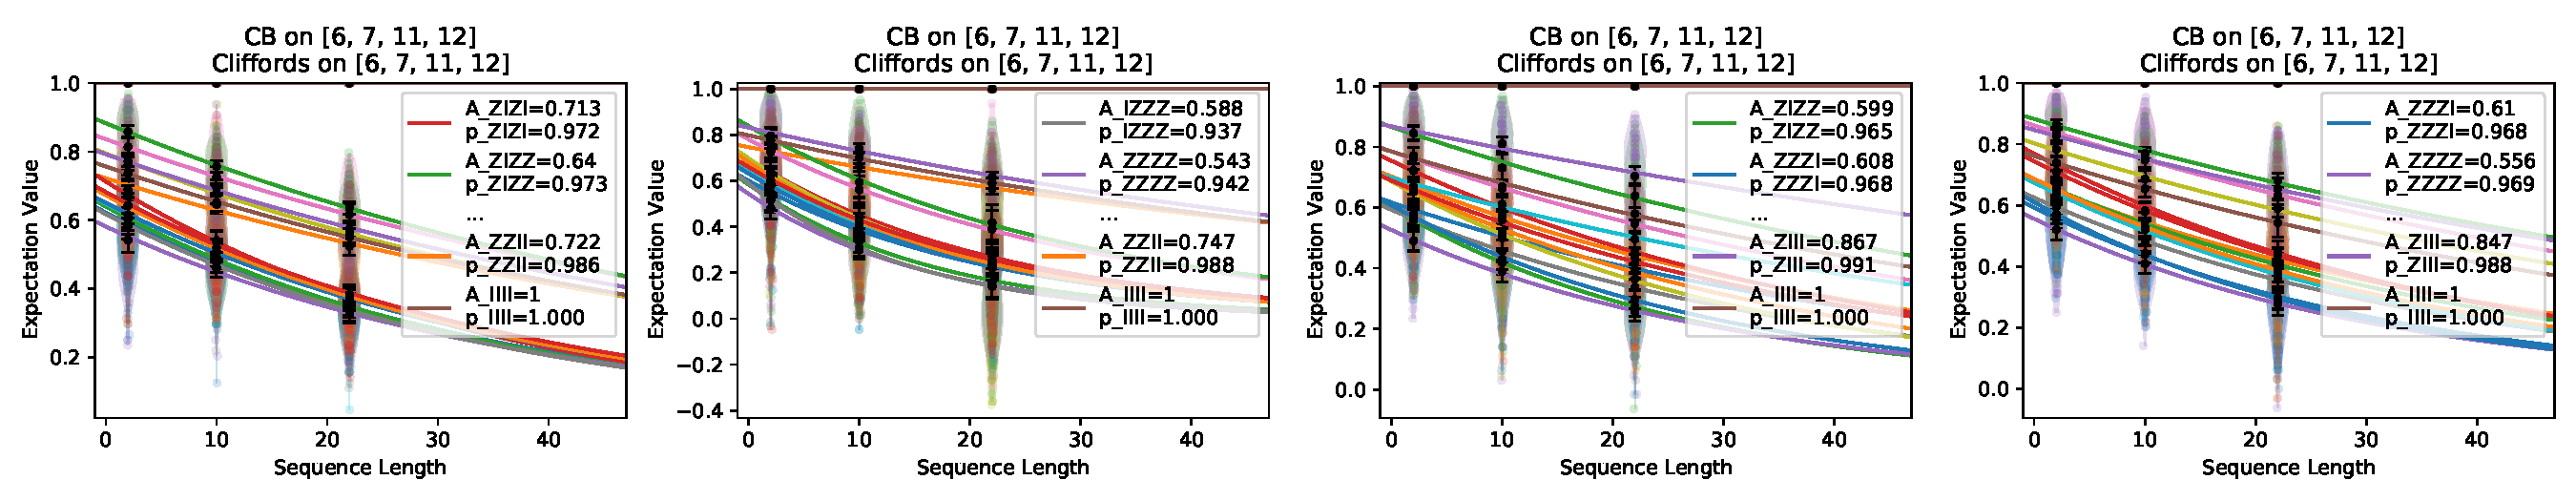
\includegraphics[scale=0.37]{4-CBRawData_24_01_2021_MorningRun_Layout2.pdf}
    \caption{Expectation values versus circuit sequence length showing the curves of the exponential Pauli decays using cycle benchmarking on the identified circuit 1 CNOT pairs on layout 2 (qubits [6, 7, 12, 11]) calculated on the morning of January 24, 2021.  Random gate sequences of length 2, 10 and 22 were selected to form the set of equations that determined each of amplitudes (A) and slopes (p) to measure of each of the Pauli decay terms.}
    \label{fig:CBRaw-1-24-2021}
%\end{figure*}

%\begin{figure*}[htpb]
    % \centering
    % \includegraphics[width=2.2\columnwidth]{final_plot.pdf}
    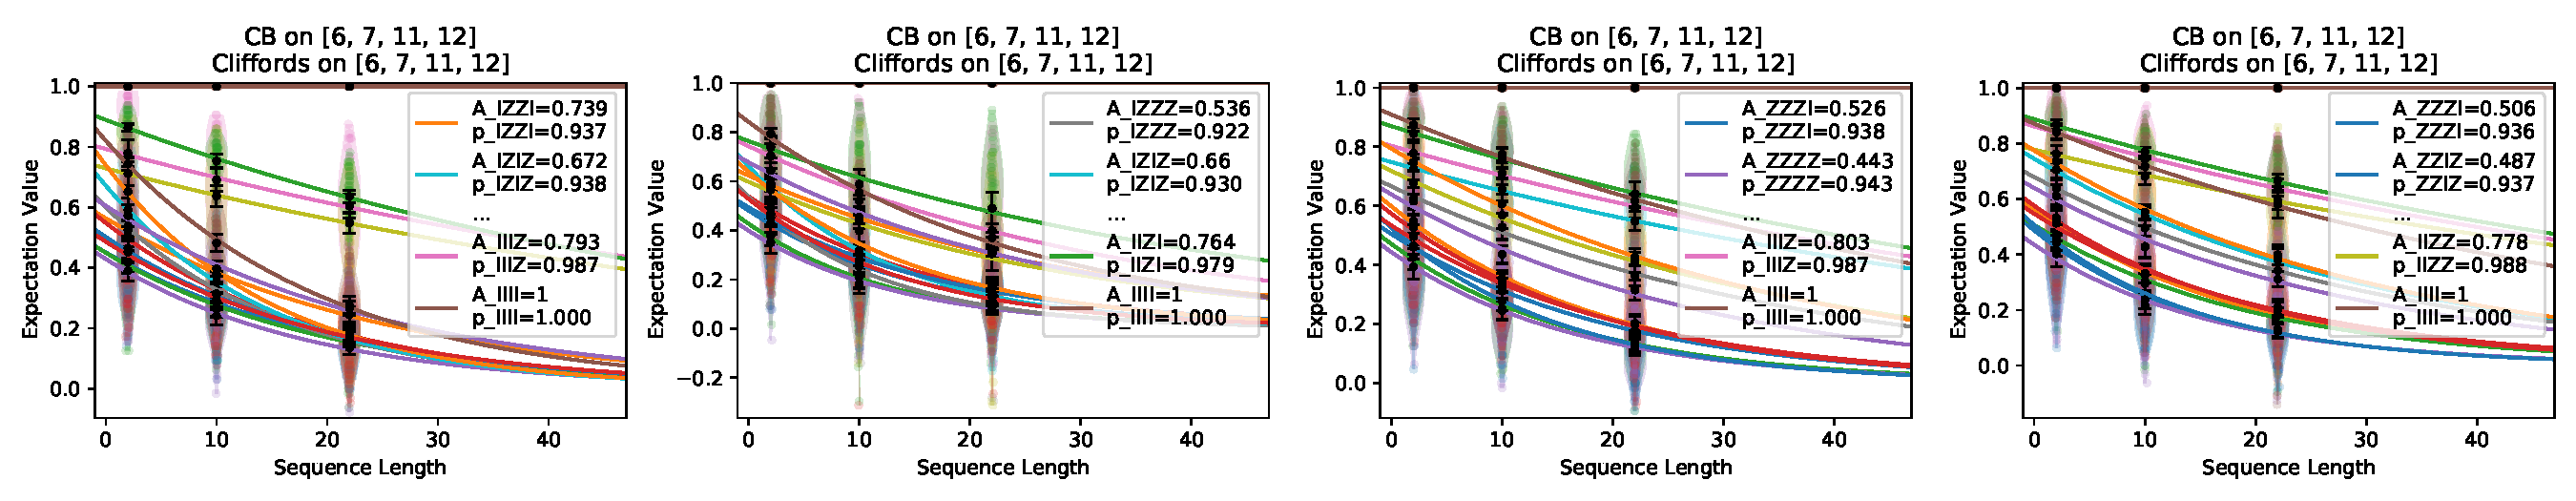
\includegraphics[scale=0.37]{4-CBRawData_29_01_2021_MorningRun_Layout2.pdf}
    \caption{Expectation values versus circuit sequence length showing the curves of the exponential Pauli decays using cycle benchmarking on the identified circuit 1 CNOT pairs on layout 2 (qubits [6, 7, 12, 11]) calculated on the morning of January 29, 2021.  Random gate sequences of length 2, 10 and 22 were selected to form the set of equations that determined each of amplitudes (A) and slopes (p) to measure of each of the Pauli decay terms.}
    \label{fig:CBRaw-1-29-2021}
%\end{figure*}

%\begin{figure*}[htpb]
    % \centering
    % \includegraphics[width=2.2\columnwidth]{final_plot.pdf}
    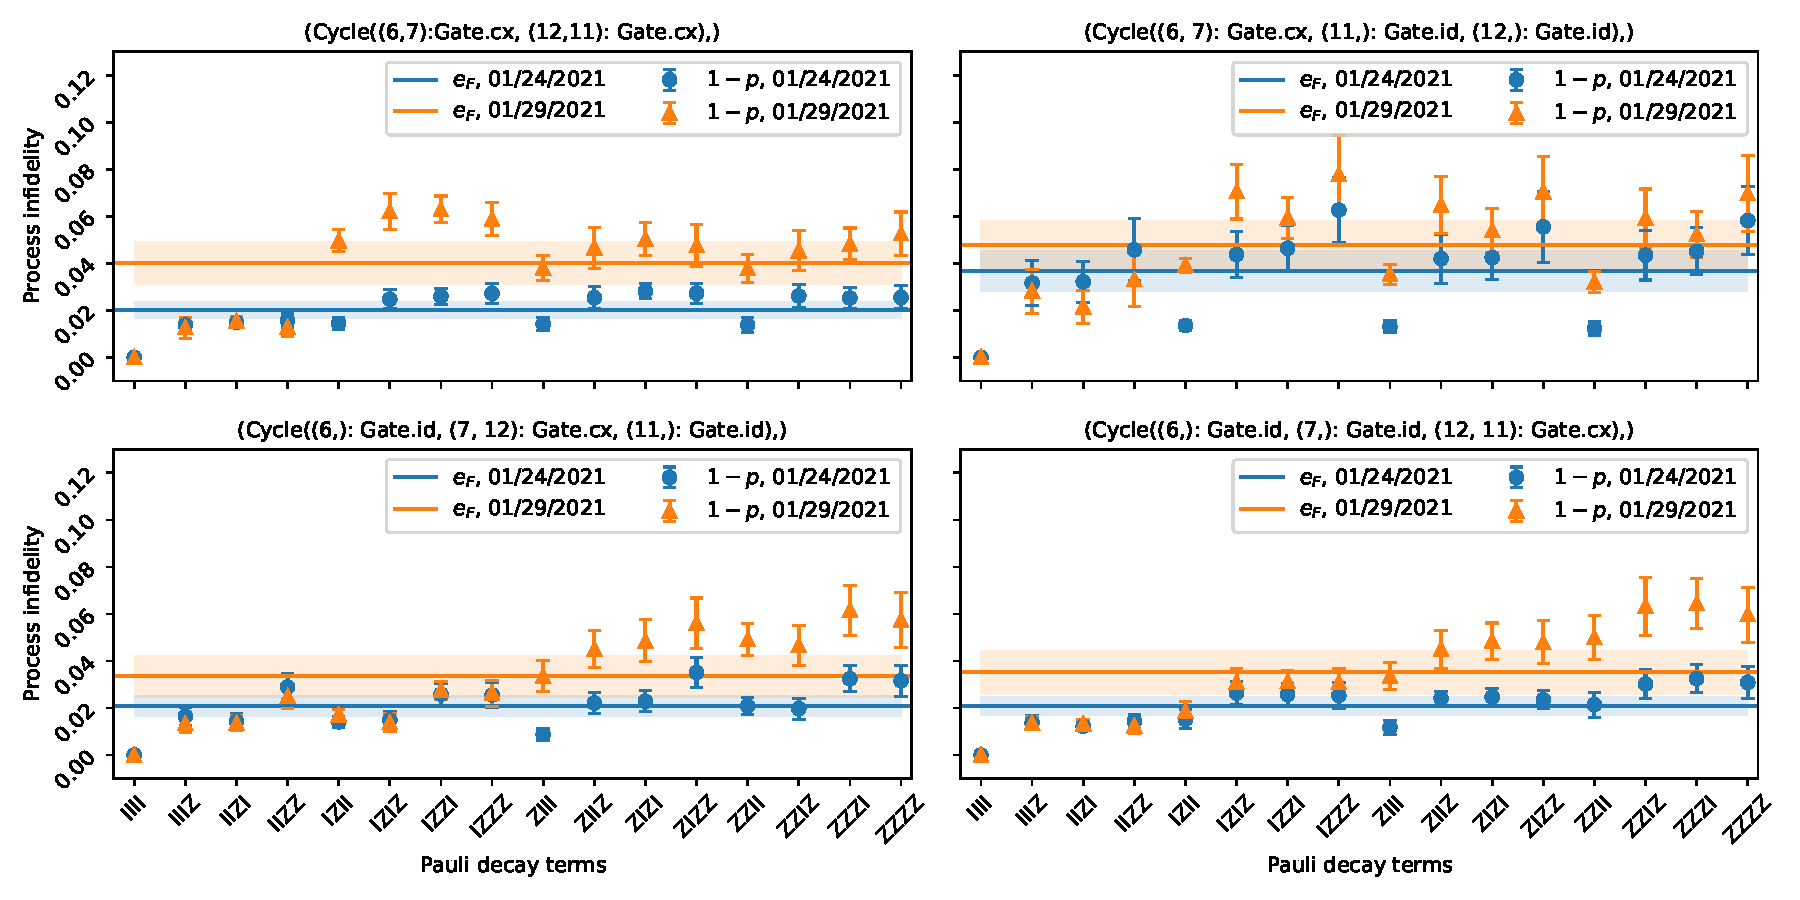
\includegraphics[scale=0.56]{CBPauliInfidelities_24_29_01_2021_MorningRun_Layout2_Cycle1_2_3_4.pdf}
    \caption{The Pauli infidelities for each hard cycle calculated for each Pauli decay term from morning run on qubits [6, 7, 12, 11] (layout 2) on days 01/24/2021 (blue lines and data points) and 01/29/2021 (orange lines and data points). The upper left graph is Cycle 1, the upper right is Cycle 2, lower left is Cycle 3 and the lower right is Cycle 4.  The total process infidelity for each of the 4 different cycles is graphed on each plot as a blue of orange solid line along with the shaded error bands for that day ($24^{th}$ in blue and $29^{th}$ in orange).  The shaded regions show the error on the process infidelity and the error bars on the markers show the statistical errors on Pauli decay terms. }
    \label{fig:PauliInfidelities24_29_Story4}
\end{figure*}










\begin{figure}[htpb]
    % \centering
    % \includegraphics[width=2.2\columnwidth]{final_plot.pdf}
    % 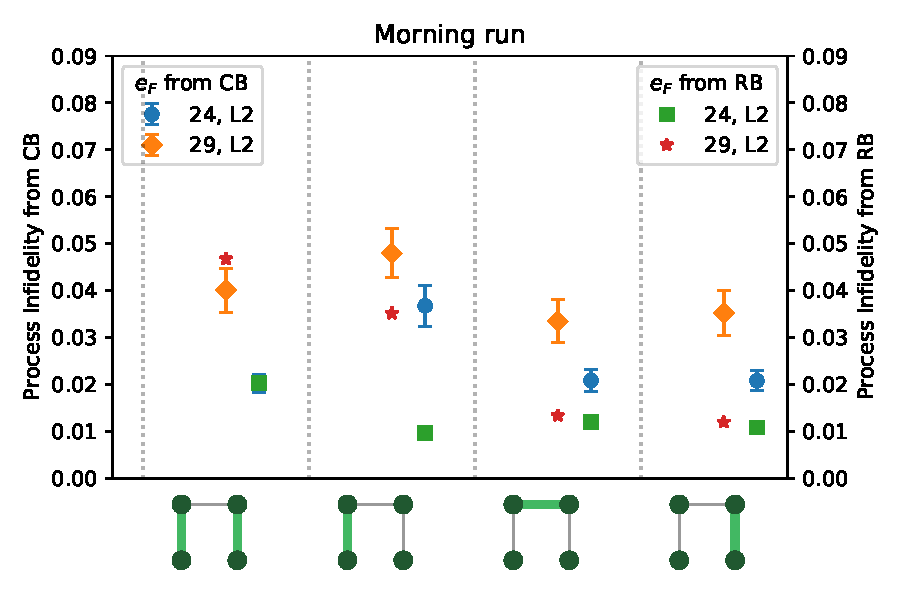
\includegraphics[scale=0.5]{ProcessInfidelities_CB_RB_Data_01_24_2021_01_292021_Layout2aligned.pdf}
    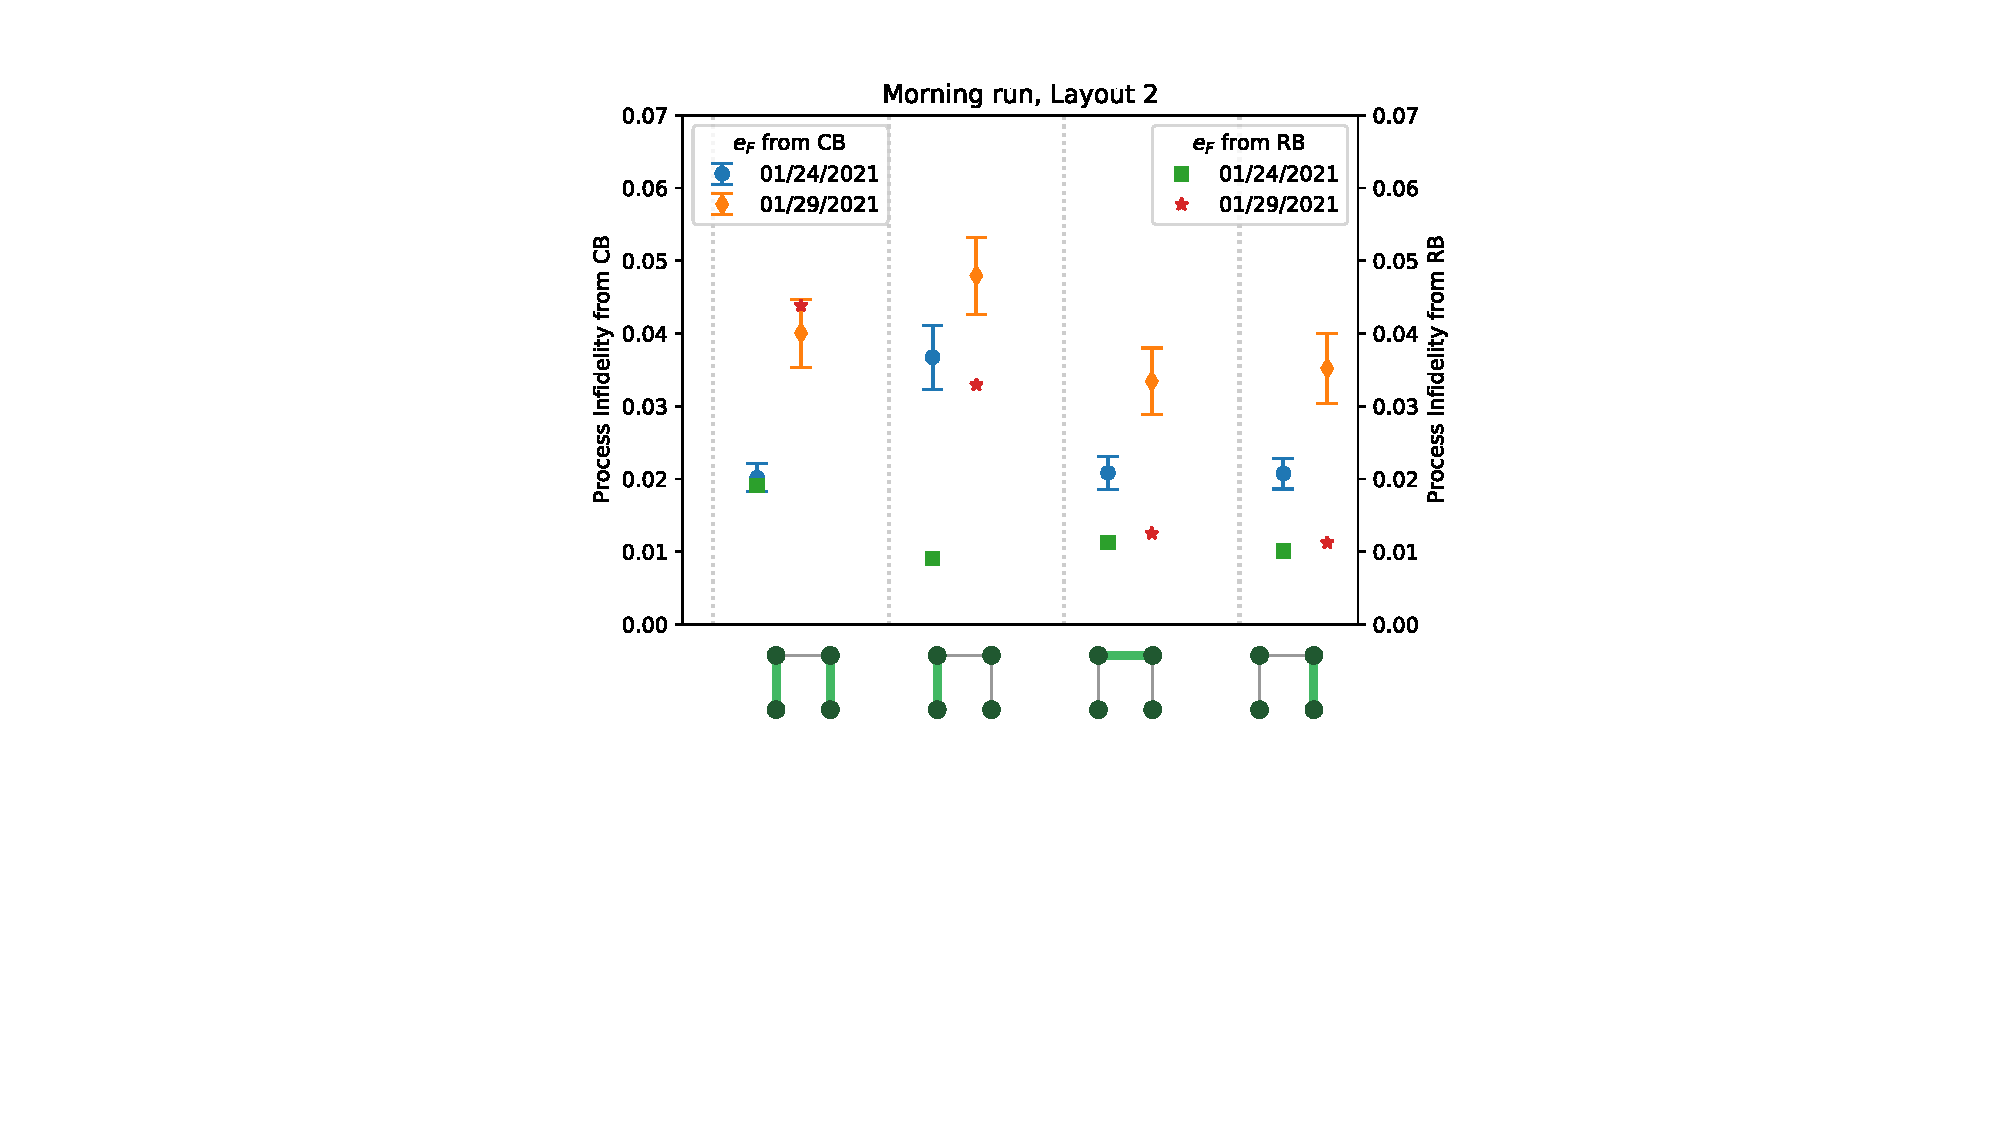
\includegraphics[scale=0.5]{ProcessInfidelitiesCB_RB_plots_24_29_morning_L2.pdf}
    \caption{The process infidelities calculated using randomized benchmarking (RB) (right axis) and cycle benchmarking (CB) (left axis) from the morning runs of circuit 1 on layout 2 (qubits [6, 7, 12, 11]) on 01/24/2021 and 01/29/2021.  the two qubit CNOT cycles 1, 2, 3, and 4 are identified along the horizontal axis from left to right}
    \label{fig:processinfidelitiesStory4}
\end{figure}
  

\begin{figure}[htpb]
    % \centering
    % \includegraphics[width=2.2\columnwidth]{final_plot.pdf}
    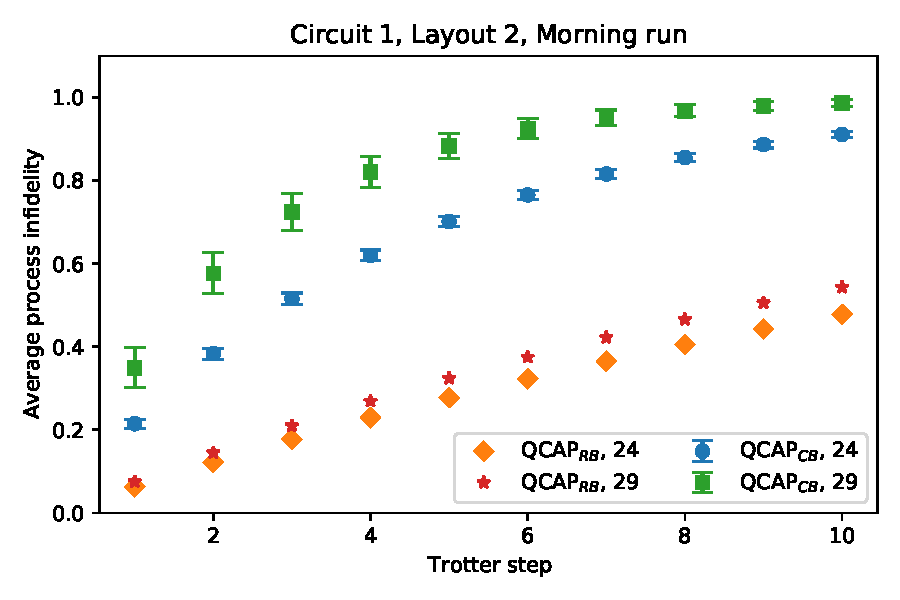
\includegraphics[scale=0.56]{QCAP_CB_RB_Data_01_24_29_2021_Layout_2C1.pdf}
    \caption{The QCAP bound as a function of number Trotter steps calculated using randomized benchmarking (QCAP$_{\text{RB}}$) (right axis) and cycle benchmarking (QCAP$_{\text{CB}}$) (left axis) from morning run of layout 2 (qubits [6, 7, 12, 11]) on days 01/24/2021 and 01/29/2021. The plotted error bars only show the statistical error.}
    \label{fig:QCAPCB_RB_Story4}
\end{figure}



\begin{figure}[htpb]
    % \centering
    % \includegraphics[width=2.2\columnwidth]{final_plot.pdf}
    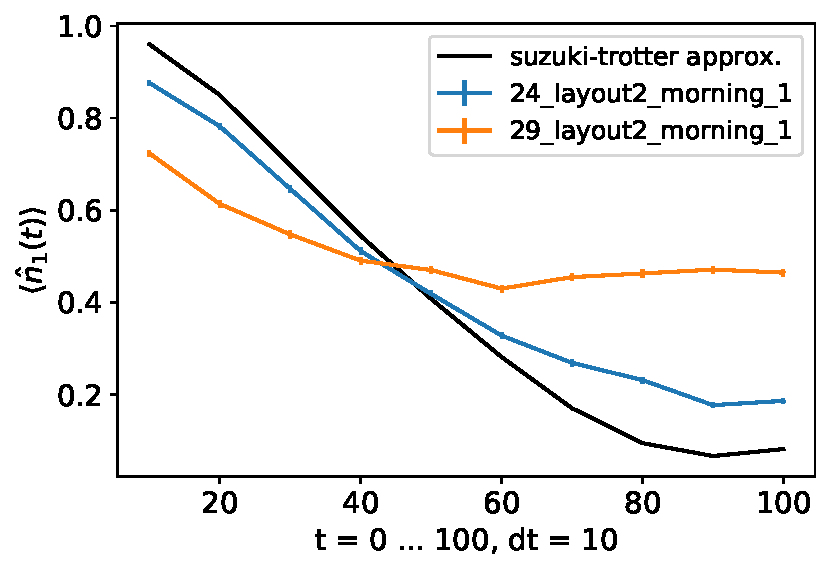
\includegraphics[scale=0.5]{TIM_[24, 29]_[layout2]_[morning]_n1.pdf}
    \caption{The particle number in site 1 calculated as a function of time from morning run of layout 2 (qubits [6, 7, 12, 11]) on days 01/24/2021 and 01/29/2021 compared to exact Suzuki-Trotter approximation.}
    \label{fig:n1_Story4}
\end{figure}



% Please add the following required packages to your document preamble:
% \usepackage{multirow}
\begin{table*}[]
\begin{tabular}{|c|c|c|c|c|c|c|}
\hline
\multicolumn{7}{|c|}{\textbf{Inter-Day Layout 2 Single Qubit CNOT Error}}                                                                                                                                                                                                                                                                   \\ \hline
                                                                                  & \textbf{Qubits} & \textbf{T1} ($\mu s $)  & \textbf{T2} ($\mu s$)  & \textbf{\begin{tabular}[c]{@{}c@{}}IBM Backend\\ Readout Error\\ 
                                                                            $10^{-2}$ \end{tabular}} & \textbf{\begin{tabular}[c]{@{}c@{}}U2\\ $10^{-4}$\end{tabular}} & \textbf{\begin{tabular}[c]{@{}c@{}}U3\\ $10^{-4}$\end{tabular}} \\ \hline
\multirow{4}{*}{\begin{tabular}[c]{@{}c@{}}01/24/2021\\ Morning Run\end{tabular}} & 6               & 67.1        & 99.9        & 2.54                                                                                 & 28.7                                                        & 5.74                                                        \\ \cline{2-7} 
                                                                                  & 7               & 94.8        & 86.8        & 2.30                                                                                 & 3.05                                                        & 6.71                                                        \\ \cline{2-7} 
                                                                                  & 12              & 97.5        & 88.5        & 3.13                                                                                 & 2.91                                                        & 5.82                                                        \\ \cline{2-7} 
                                                                                  & 11              & 95.1        & 71.6        & 3.55                                                                                 & 4.44                                                        & 8.88                                                        \\ \hline
\multirow{4}{*}{\begin{tabular}[c]{@{}c@{}}01/29/2021\\ Morning Run\end{tabular}} & 6               & 24.1        & 4.97        & 9.19                                                                                 & 25.0                                                        & 50.0                                                        \\ \cline{2-7} 
                                                                                  & 7               & 78.8        & 103.4       & 2.84                                                                                 & 3.97                                                        & 7.94                                                        \\ \cline{2-7} 
                                                                                  & 12              & 80.8        & 114.6       & 3.47                                                                                 & 3.49                                                        & 6.98                                                        \\ \cline{2-7} 
                                                                                  & 11              & 48.4        & 87.8        & 3.22                                                                                 & 4.64                                                        & 9.29                                                        \\ \hline
\end{tabular}


\label{table:Single-qubit-gate-error-layout2-on-1-24-and-1-29} 
\caption{Values for single qubit errors for Layout 2 (qubits[6,7,12,11]) extracted from the recorded IBM back-end properties immediately after IBM completed a full re-calibration of the Boeblingen quantum chip on the morning of January 24, 2021 and January 29, 2021 and the error values for the basis gates U2 and U3.}
\end{table*}





% Please add the following required packages to your document preamble:
% \usepackage{multirow}
% \usepackage[table,xcdraw]{xcolor}
% If you use beamer only pass "xcolor=table" option, i.e. \documentclass[xcolor=table]{beamer}
\begin{table*}[]
\begin{tabular}{|
>{\columncolor[HTML]{FFFFFF}}c |l|
>{\columncolor[HTML]{FFFFFF}}c |
>{\columncolor[HTML]{FFFFFF}}c |}
\hline
\multicolumn{4}{|c|}{\cellcolor[HTML]{FFFFFF}{\color[HTML]{333333} \textbf{Layout 2 Inter-Day Two-Qubit Gate Error}}}                                                                                                                  \\ \hline
\textbf{}                                                                                                  & \textbf{Cycle} & \textbf{Qubits}                 & \textbf{\begin{tabular}[c]{@{}c@{}}CNOT Error\\ $10^{-2}$ \end{tabular}} \\ \hline
\cellcolor[HTML]{FFFFFF}                                                                                   & 2              & [6,7]                           & 2.94                                                                  \\ \cline{2-4} 
\cellcolor[HTML]{FFFFFF}                                                                                   & 3              & [7,12]                          & 1.67                                                                  \\ \cline{2-4} 
\multirow{-3}{*}{\cellcolor[HTML]{FFFFFF}\begin{tabular}[c]{@{}c@{}}01/24/2021\\ Morning Run\end{tabular}} & 4              & [12,11]                         & 1.66                                                                  \\ \hline
\cellcolor[HTML]{FFFFFF}                                                                                   & 2              & \cellcolor[HTML]{FFFFFF}[6,7]   & 3.84                                                                  \\ \cline{2-4} 
\cellcolor[HTML]{FFFFFF}                                                                                   & 3              & \cellcolor[HTML]{FFFFFF}[7,12]  & 2.67                                                                  \\ \cline{2-4} 
\multirow{-3}{*}{\cellcolor[HTML]{FFFFFF}\begin{tabular}[c]{@{}c@{}}01/29/2021\\ Morning Run\end{tabular}} & 4              & \cellcolor[HTML]{FFFFFF}[12,11] & 2.82                                                                  \\ \hline
\end{tabular}
\label{table:Two-qubit-gate-error-layout2-on-1-24-and-1-29} 
\caption{Values for two qubit error pairs [6, 7], [7,12], [12, 11] extracted from the recorded IBM back-end properties immediately after IBM completed a full re-calibration of the Boeblingen quantum chip on the morning of January 24, 2021 and January 29, 2021 \textbf{mention error bars in text} and the error values for the two qubit pairs from cycle 2, 3, and 4 from the cycle benchmarking computations.}
\end{table*}




%==============================





% Figure \ref{fig:4-CBRawData_24_01_2021_MorningRun_Layout2}
%for the 24th.  Figure \ref{fig:4-CBRawData_29_01_2021_MorningRun_Layout2} for the 29th

%\begin{figure*}[ht!]
    % \centering
    % \includegraphics[width=2.2\columnwidth]{final_plot.pdf}
%    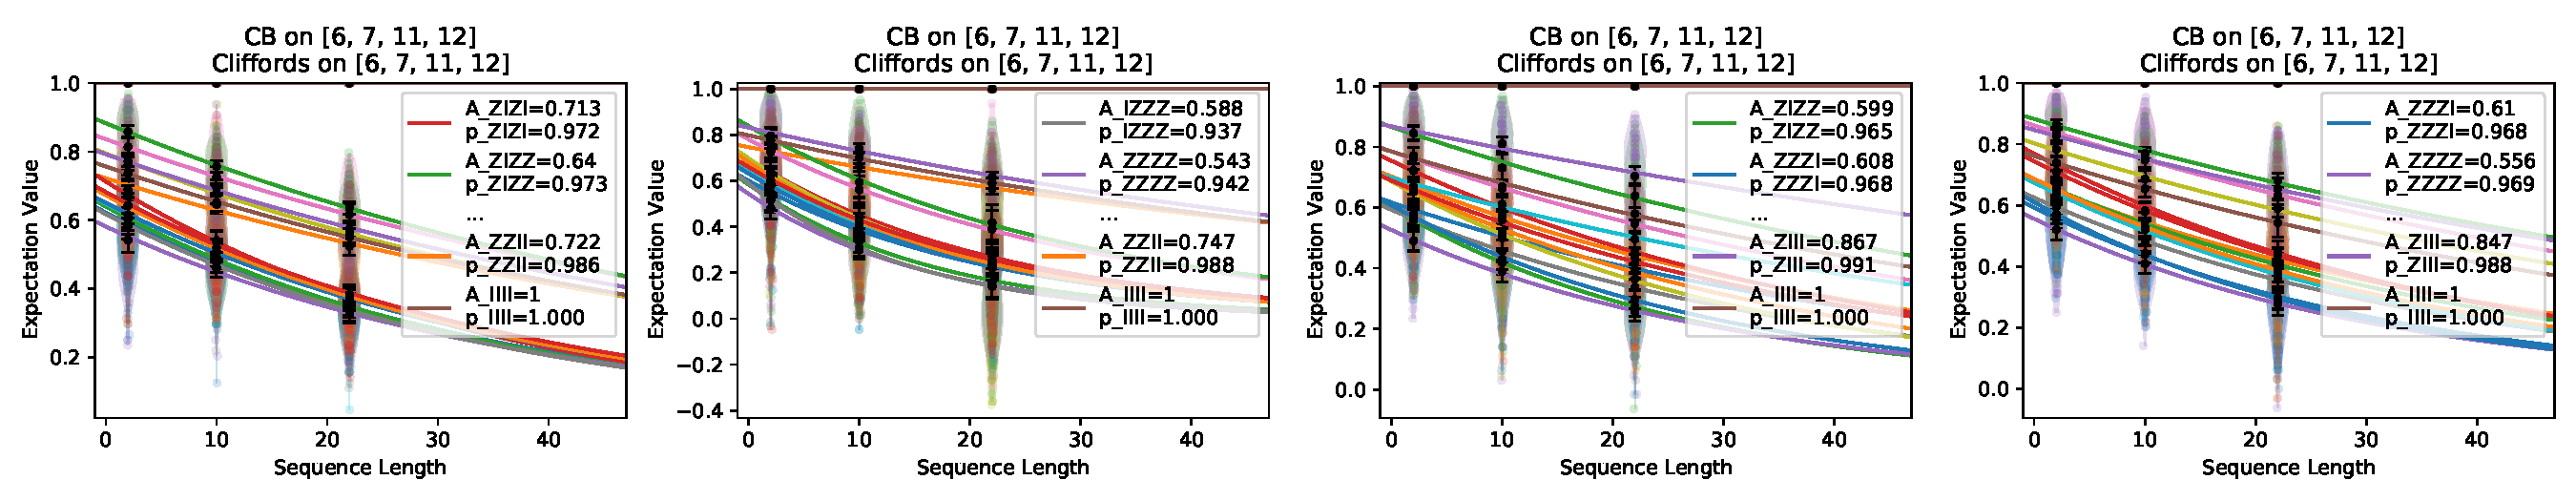
\includegraphics[scale=0.4]{4-CBRawData_24_01_2021_MorningRun_Layout2.pdf}
%    \caption{Expectation values of the Pauli group versus sequence length plotted for random Pauli gate sequences of length 2, 10 and 22 showing decay curves for all I and Z gate combinations with both amplitude (A) and slope (p) from morning run of layout 2 (qubits [6, 7, 12, 11]) on 01/24/2021.}
%    \label{fig:4-CBRawData_24_01_2021_MorningRun_Layout2}
%\end{figure*}

%\begin{figure*}[ht!]
    % \centering
    % \includegraphics[width=2.2\columnwidth]{final_plot.pdf}
%    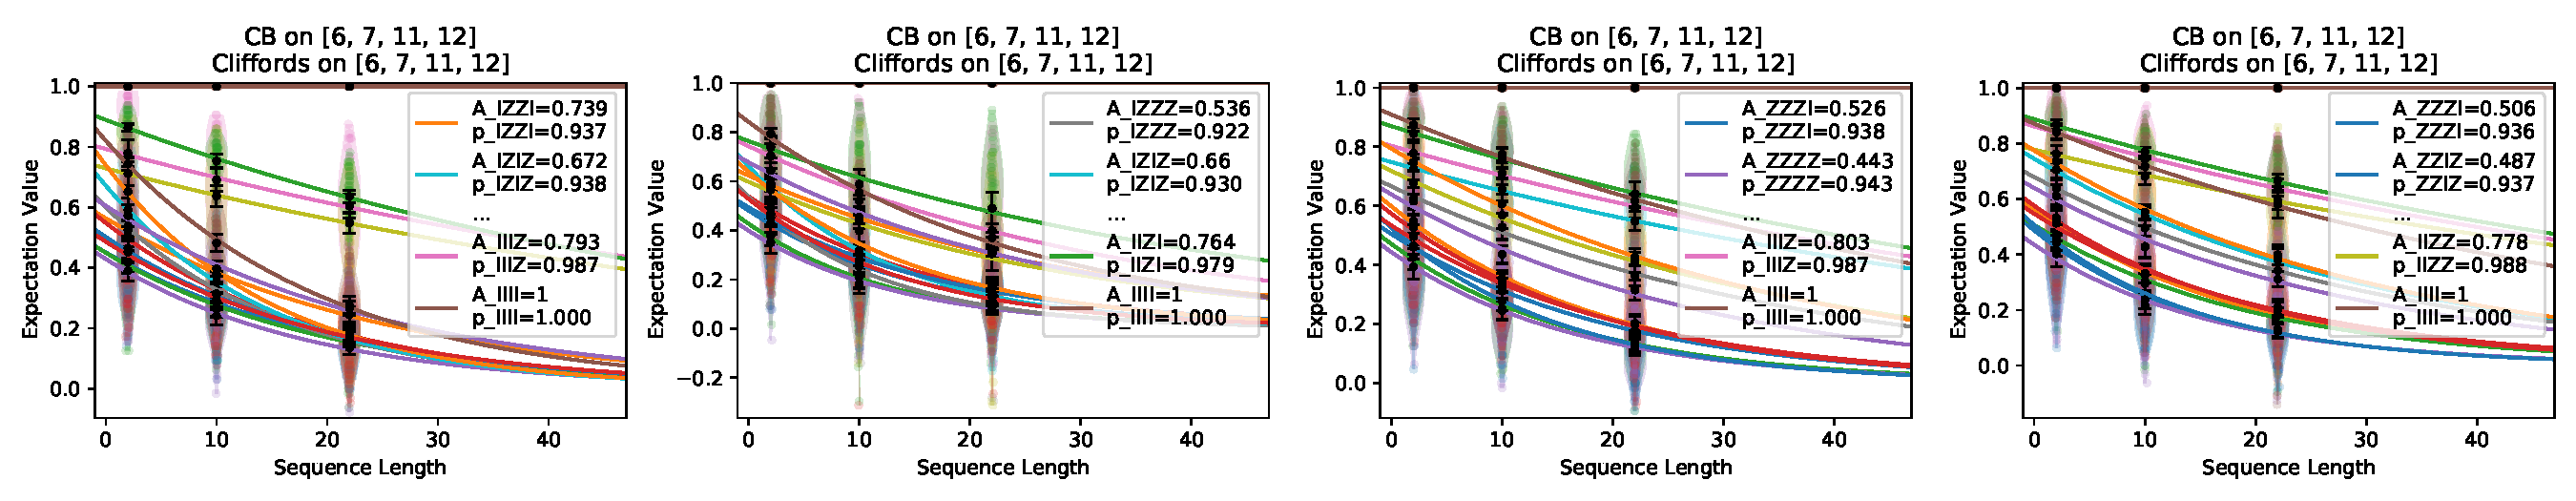
\includegraphics[scale=0.4]{4-CBRawData_29_01_2021_MorningRun_Layout2.pdf}
%    \caption{Expectation values of the Pauli group versus sequence length plotted for random Pauli gate sequences of length 2, 10 and 22 showing decay curves for all I and Z gate combinations with both amplitude (A) and slope (p) from morning run of layout 2 (qubits [6, 7, 12, 11]) on 01/29/2021.}
%    \label{fig:4-CBRawData_29_01_2021_MorningRun_Layout2}
%\end{figure*}













%======================================================================================
%======================================================================================
%======================================================================================



\subsection{Intra-day Calibration Drift}
\label{intra-day-analysis}

We also observed intra-day calibration drift throughout both the morning and night time periods when measurements were being recorded using the Boeblingen hardware platform.  Examples of this intra-day calibration drift can be seen with both the TIM and cycle benchmarking data using circuit 1 applied to the qubits on layout2 for runs done on January 27, 2021 and January 30, 2021.  The data analysis for both days follows the same methodology and procedures described in the previous section discussing inter-day calibration drift.  

For the analysis of the January 27th data the morning run was selected as the baseline on which to measure the intra-day drift.  Using cycle benchmarking for the 4 different cycles from circuit 1, expectation values versus sequence length were measured using Clifford sequences of length 2, 10 and 22 and a set of equations were solved to find Pauli decay terms amplitude (A) and slope (p) from these exponential decays.  The individual process infidelity values and error bars for each Pauli term for each cycle was then plotted in Figure \ref{fig:PauliInfidelities27Morning_Story6}.   A similar set of measurements were performed using the data recorded on January 27, 2021 after the 2 qubit night re-calibration by IBM (Figure~\ref{fig:PauliInfidelities27Night_Story6}


\begin{figure*}[htpb]
    % \centering
    % \includegraphics[width=2.2\columnwidth]{final_plot.pdf}
    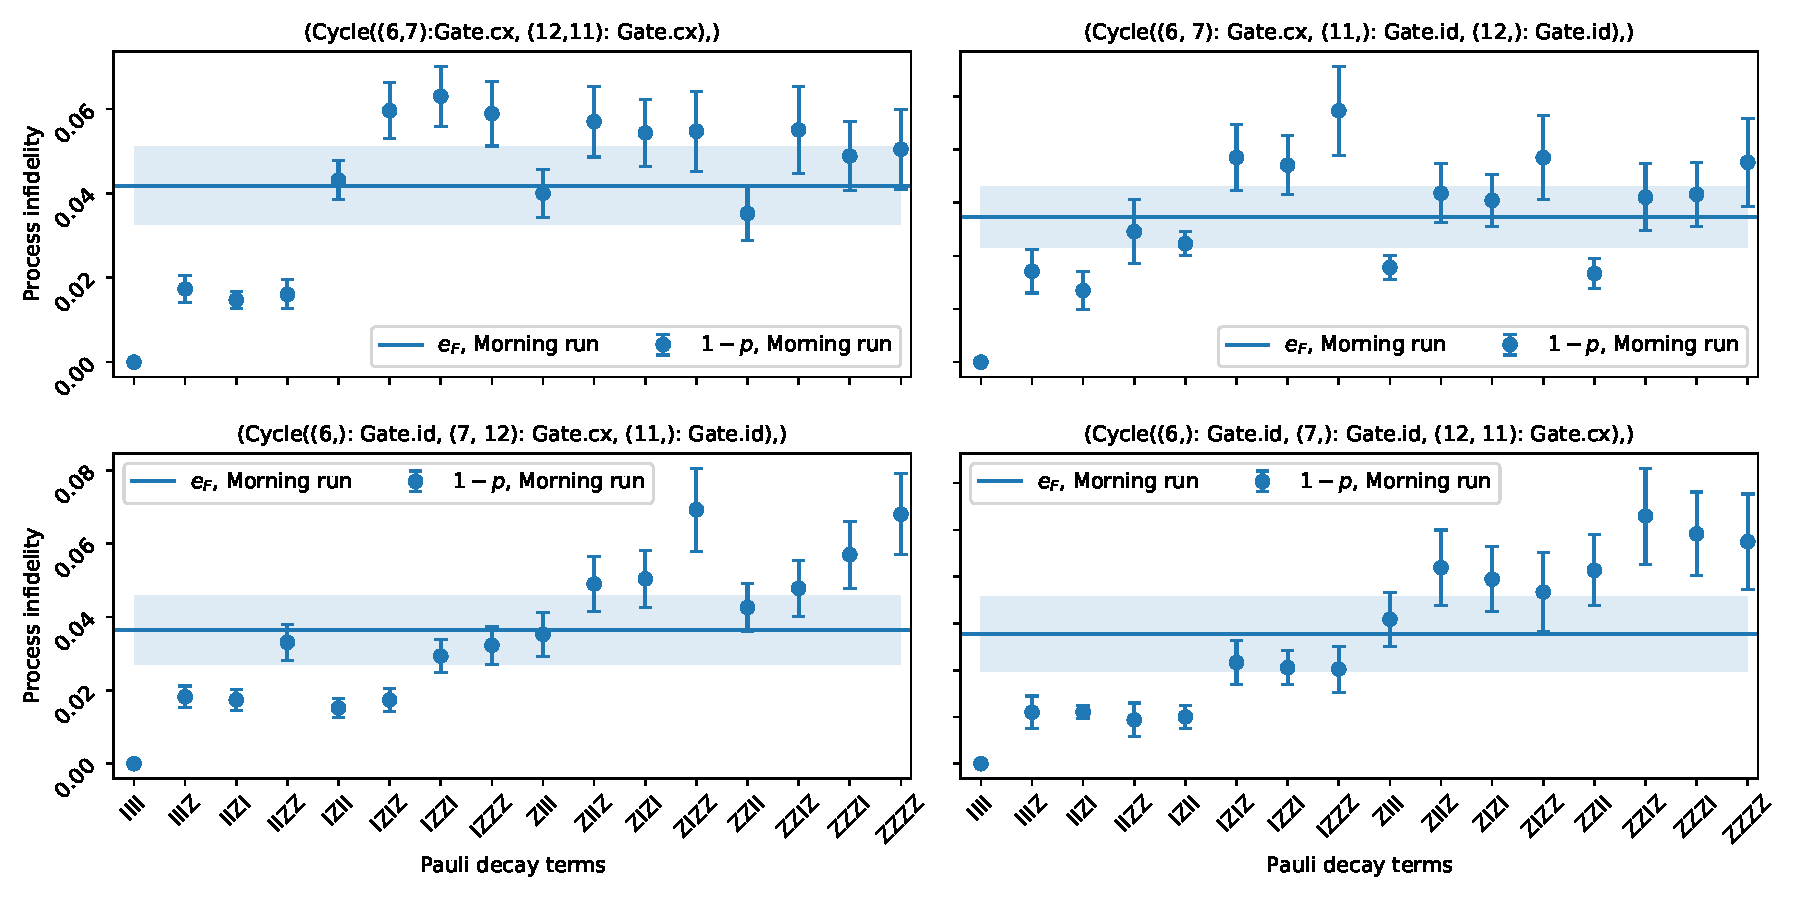
\includegraphics[scale=0.56]{CBPauliInfidelities_27_01_2021_MorningRun_Layout2_Cycle1_2_3_4.pdf}
    \caption{The Pauli infidelities for each hard cycle calculated for each Pauli decay term from morning run of layout 2 (qubits [6, 7, 12, 11]) on January 27, 2021. The shaded regions show the error on the process infidelity and the error bars on the markers show the statistical errors on Pauli decay terms. }
    \label{fig:PauliInfidelities27Morning_Story6}
\end{figure*}

\begin{figure*}[htpb]
    % \centering
    % \includegraphics[width=2.2\columnwidth]{final_plot.pdf}
    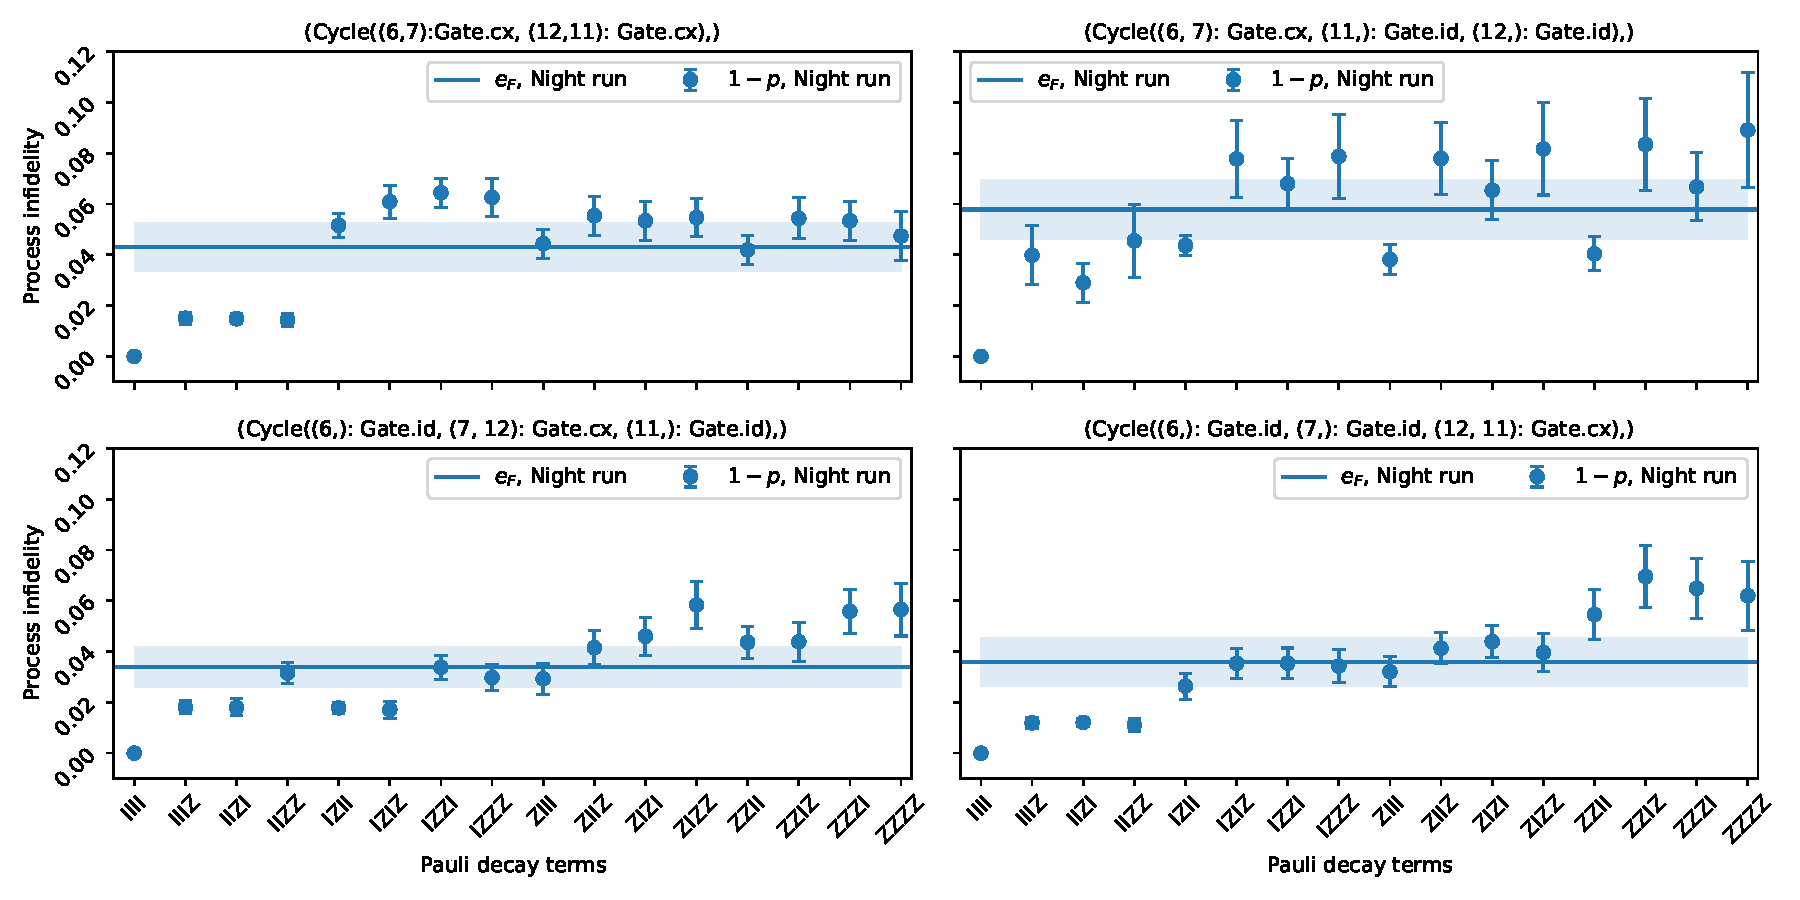
\includegraphics[scale=0.56]{CBPauliInfidelities_27_01_2021_NightRun_Layout2_Cycle1_2_3_4.pdf}
    \caption{The Pauli infidelities for each hard cycle calculated for each Pauli decay term from night run of layout 2 (qubits [6, 7, 12, 11]) on January 27, 2021. The shaded regions show the error on the process infidelity and the error bars on the markers show the statistical errors on Pauli decay terms. }
    \label{fig:PauliInfidelities27Night_Story6}
\end{figure*}
 
After both the individual process infidelities were calculated from the January 27th morning and night data the process infidelities for cycles 1, 2, 3, and 4 were then plotted on the same graph with the process infidelities from randomized benchmarking measurements ( Figure~\ref{fig:processinfidelitiesStory6} )

From the January 27th data the detailed variances between the morning and night 2 qubit re-calibrations of qubits 6, 7, 11, and 12 can be seen when comparing the Pauli infidelities for each hard cycle calculated for each Pauli decay term from morning run of layout 2 (qubits [6, 7, 12, 11]) on 01/27/2021 
Fig.~\ref{fig:PauliInfidelities27Morning_Story6}, 
the night run shown in Fig.~\ref{fig:PauliInfidelities27Night_Story6} 
and the overall process infidelity for cycles 1, 2, 3, and 4 in Fig.~\ref{fig:processinfidelitiesStory6} for January 27th.


\begin{figure}[htpb]
    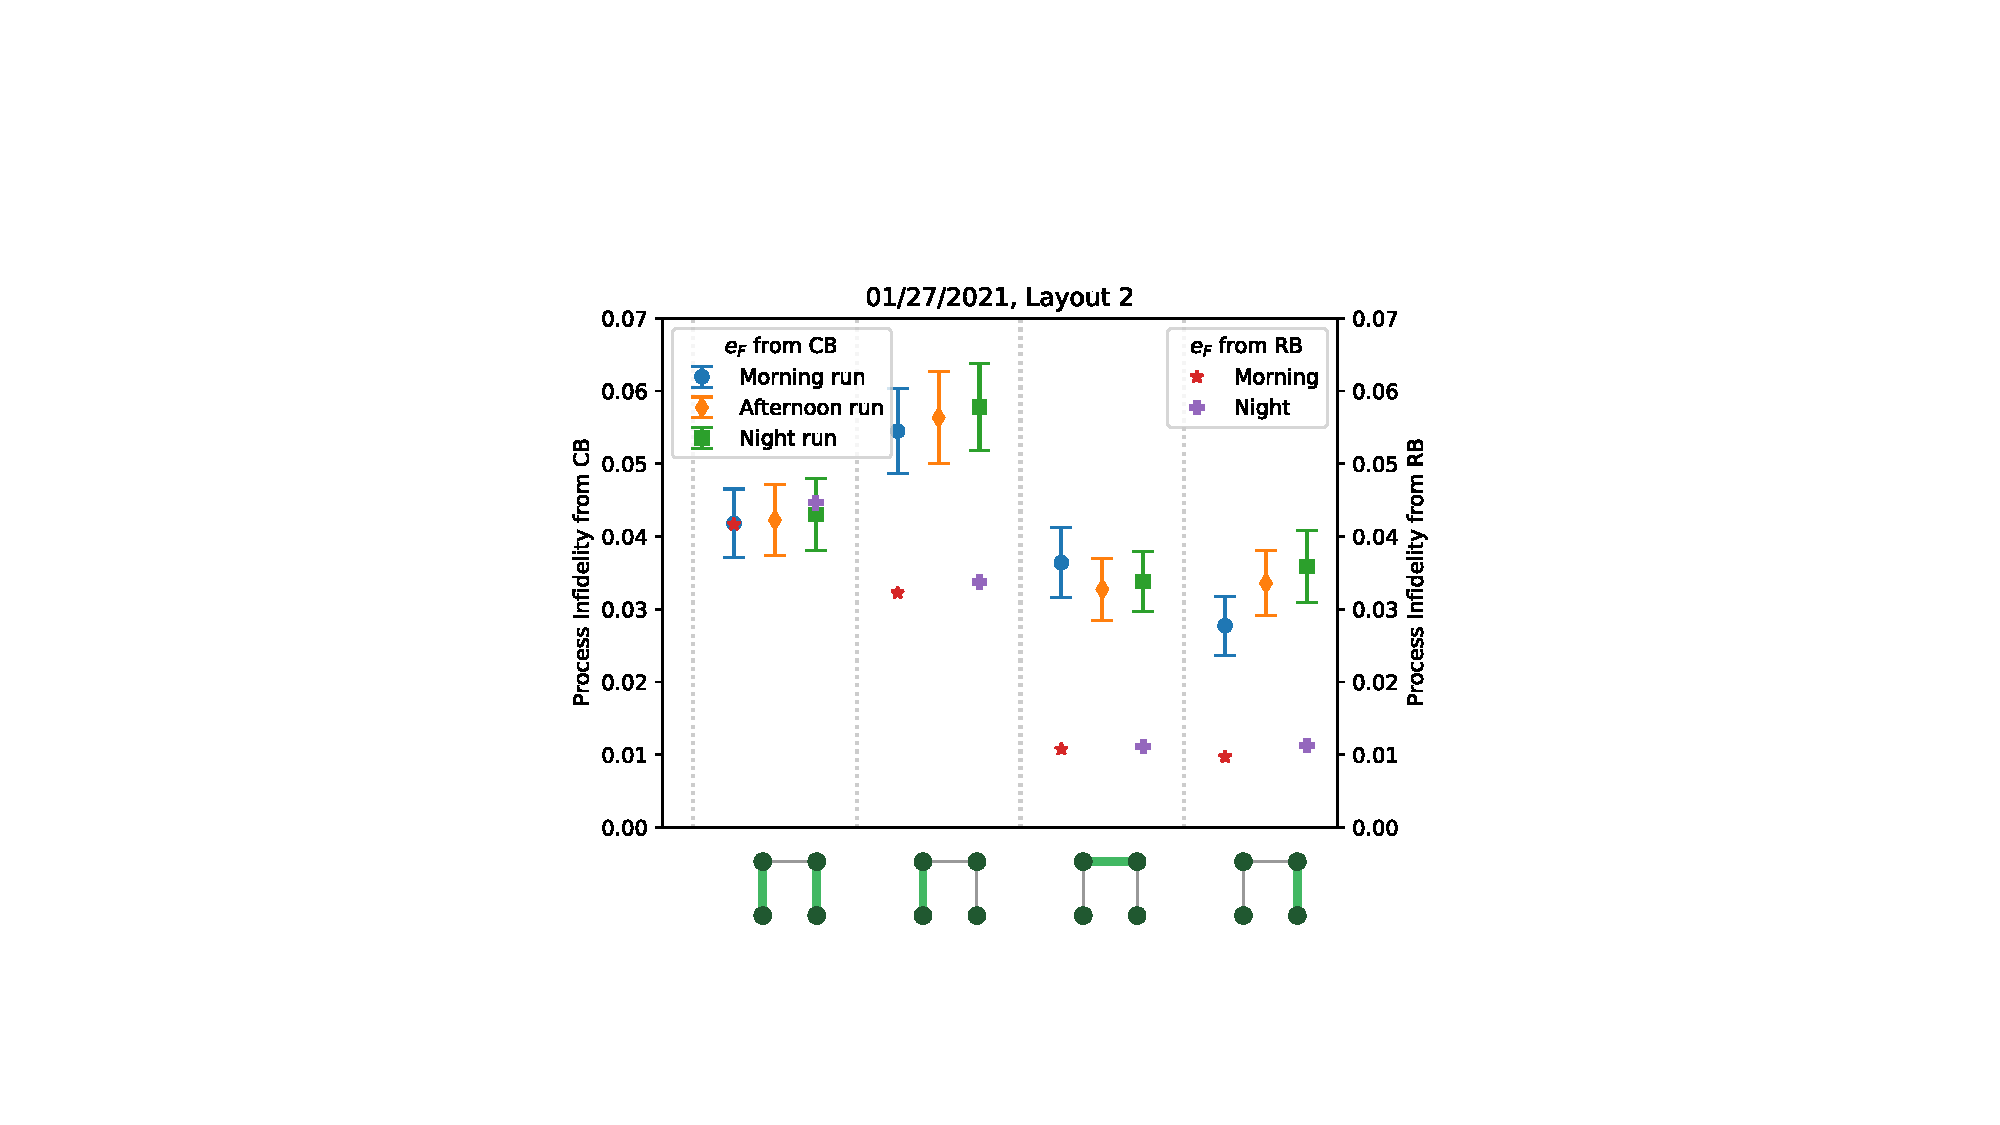
\includegraphics[scale=0.56]{ProcessInfidelitiesCB_RB_plots_27_morning_afternoon_night_L2.pdf}
    \caption{The process infidelities for cycles  1, 2, 3, and 4 calculated using randomized benchmarking (RB) (right axis) and cycle benchmarking (CB) (left axis) from morning, afternoon and night runs of layout 2 [qubits 6, 7, 12, 11] on January 27, 2021.}
    \label{fig:processinfidelitiesStory6}
\end{figure}

Finally, using cycle benchmarking for the entire circuit 1 the QCAP bound as a function of number Trotter steps was calculated and compared to the randomized benchmarking data taken from the IBM backend properties for January 27, 2021 (Fig.~\ref{fig:QCAPCB_RB_Story6}).

\begin{figure}[htpb]
    % \centering
    % \includegraphics[width=2.2\columnwidth]{final_plot.pdf}
    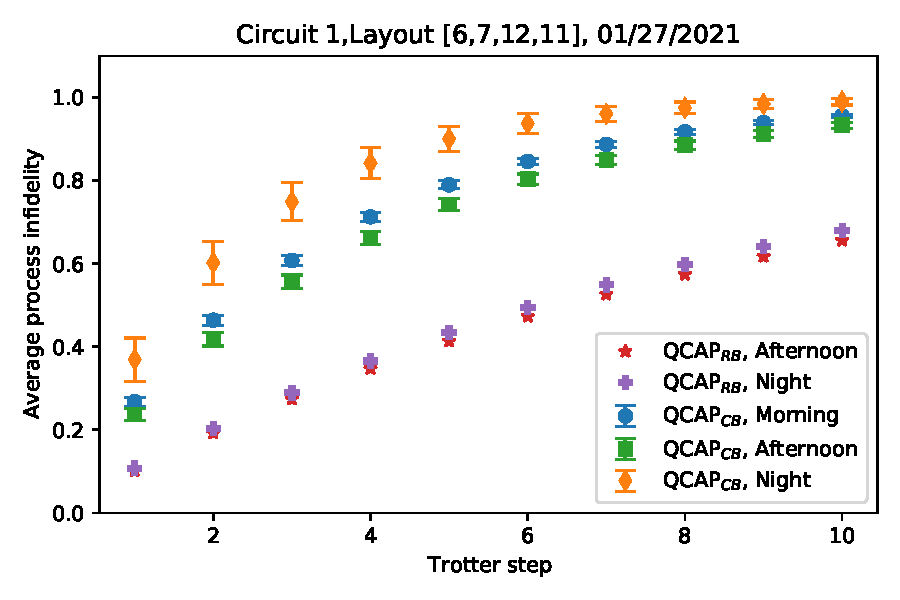
\includegraphics[scale=0.56]{QCAP_CB_RB_Data_01_27_2021_Layout_2C1.pdf}
    \caption{The QCAP bound as a function of number Trotter steps calculated using randomized benchmarking (QCAP$_{\text{RB}}$) (right axis) and cycle benchmarking (QCAP$_{\text{CB}}$) (left axis) from morning, afternoon and night runs of layout 2 [qubits 6, 7, 12, 11] on  01/27/2021.}
    \label{fig:QCAPCB_RB_Story6}
\end{figure}

The particle number in site 1 was calculated from the TIM Hamiltonian computations for the morning, afternoon and evening of January 27, 2021 and plotted in Fig.~\ref{fig:n1_Story6}.


\begin{figure}[htpb]
    % \centering
    % \includegraphics[width=2.2\columnwidth]{final_plot.pdf}
    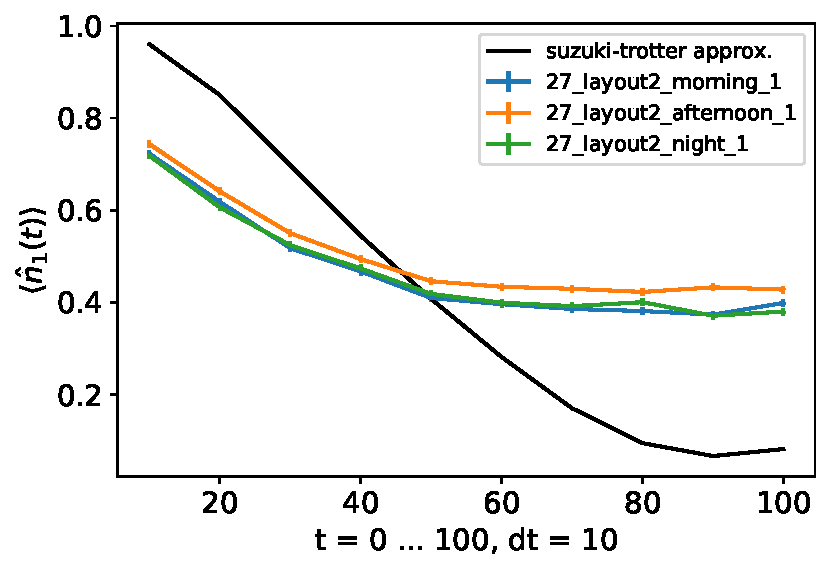
\includegraphics[scale=0.55]{TIM_[27]_[layout2]_[morning, afternoon, night]_n1.pdf}
    \caption{The particle number in site 1 calculated as a function of time from morning, afternoon. and night run of layout 2 [qubits 6, 7, 12, 11] on days January 27, 2021 compared to exact Suzuki-Trotter approximation.}
    \label{fig:n1_Story6}
\end{figure}




%=============================
%  January 30
%=============================

A similar set of calculations applied to the data from January 27th was repeated for data acquired on January 30th.  Using cycle benchmarking for the 4 different cycles from circuit 1 were run with expectation values versus sequence length were measured using Clifford sequences of length 2, 10 and 22.  The resulting set of equations were solved to find Pauli decay terms amplitude (A) and slope (p) from these exponential decays.  The individual process infidelity values and error bars for each Pauli term for each cycle was then plotted in Figure \ref{fig:PauliInfidelities30Morning_Story7} and Figures \ref{fig:PauliInfidelities30Night_Story7}

After both the individual process infidelities were calculated from the January 30th morning and night data the process infidelities for cycles 1, 2, 3, and 4 were then plotted on the same graph with the process infidelities from randomized benchmarking measurements ( Figure~\ref{fig:processinfidelitiesStory7} )

From the January 30th data the detailed variances between the morning and night 2 qubit re-calibrations of qubits 6, 7, 11, and 12 can be seen when comparing the Pauli infidelities for each hard cycle calculated for each Pauli decay term from morning run of layout 2 (qubits [6, 7, 12, 11]) on 01/30/2021 
Fig.~\ref{fig:PauliInfidelities30Morning_Story7}, 
the night run shown in Fig.~\ref{fig:PauliInfidelities30Night_Story7} 
and the overall process infidelity for cycles 1, 2, 3, and 4 in Fig.~\ref{fig:processinfidelitiesStory7} for January 30th.

Finally, using cycle benchmarking for the entire circuit 1 the QCAP bound as a function of number Trotter steps was calculated and compared to the randomized benchmarking data taken from the IBM backend properties for January 27, 2021 (Fig.~\ref{fig:QCAPCB_RB_Story7}).

The particle number in site 1 was calculated from the TIM Hamiltonian computations for the morning, afternoon and evening of January 27, 2021 and plotted in Fig.~\ref{fig:n1_Story7}.




\begin{figure*}[htpb]
    % \centering
    % \includegraphics[width=2.2\columnwidth]{final_plot.pdf}
    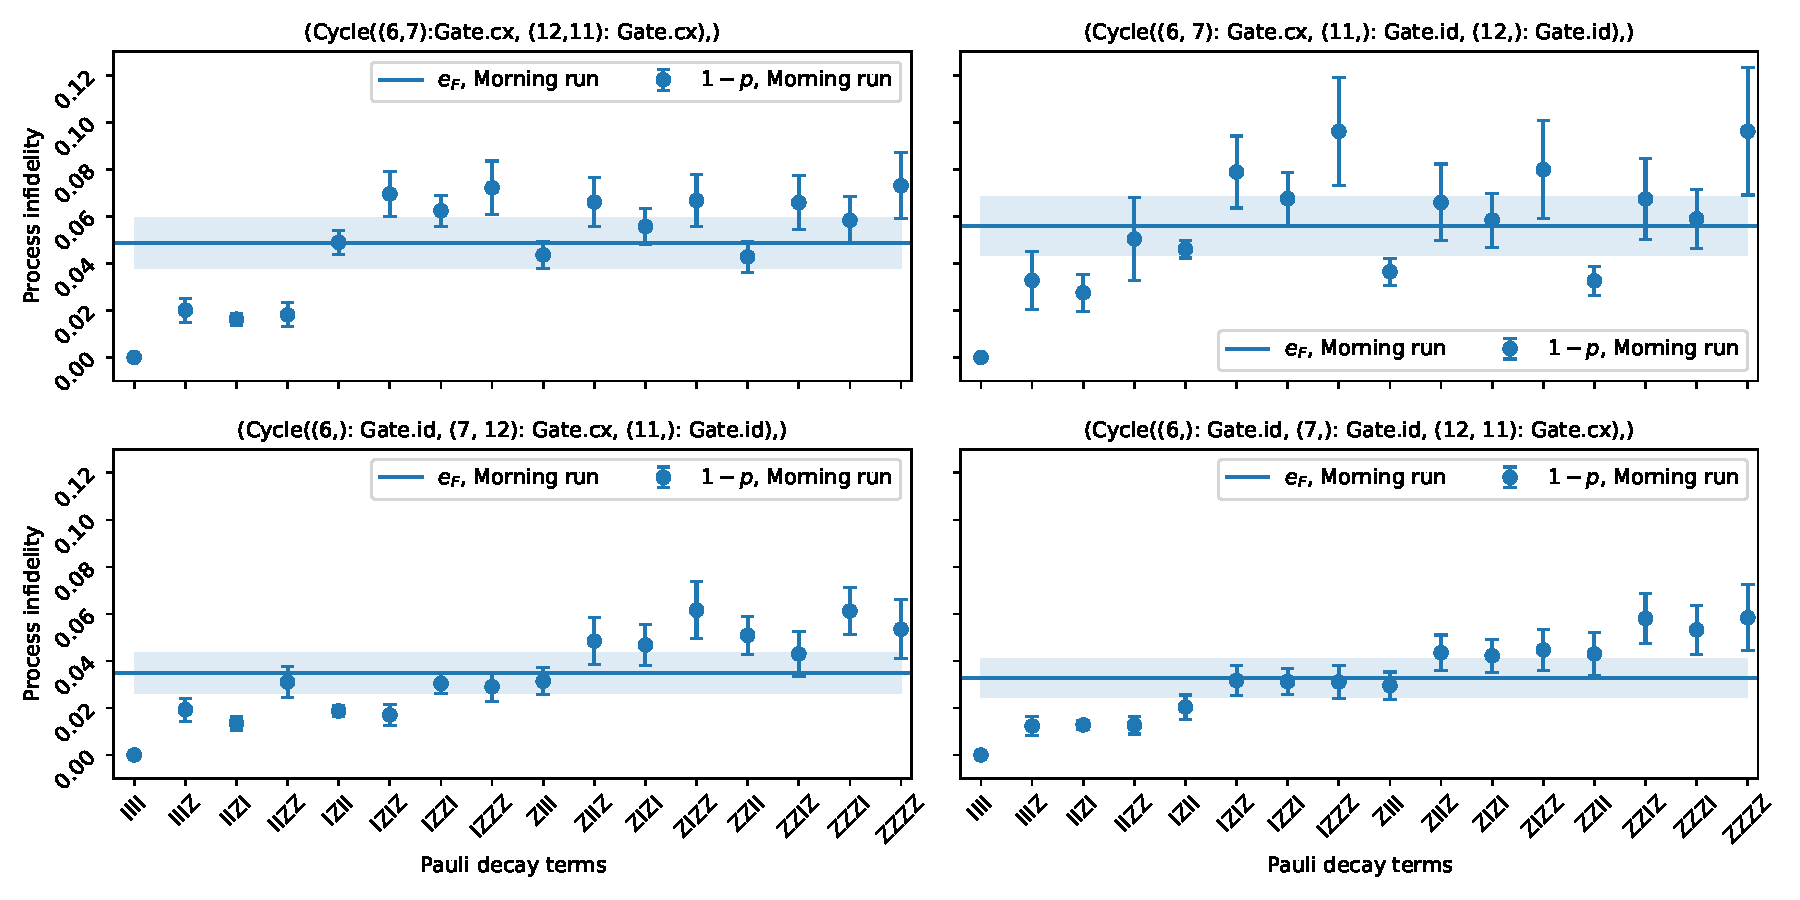
\includegraphics[scale=0.56]{CBPauliInfidelities_30_01_2021_MorningRun_Layout2_Cycle1_2_3_4.pdf}
    \caption{The Pauli infidelities for each hard cycle calculated for each Pauli decay term from morning run of layout 2 (qubits [6, 7, 12, 11]) on day 01/30/2021. The shaded regions show the error on the process infidelity and the error bars on the markers show the statistical errors on Pauli decay terms. }
    \label{fig:PauliInfidelities30Morning_Story7}
\end{figure*}



\begin{figure*}[htpb]
    % \centering
    % \includegraphics[width=2.2\columnwidth]{final_plot.pdf}
    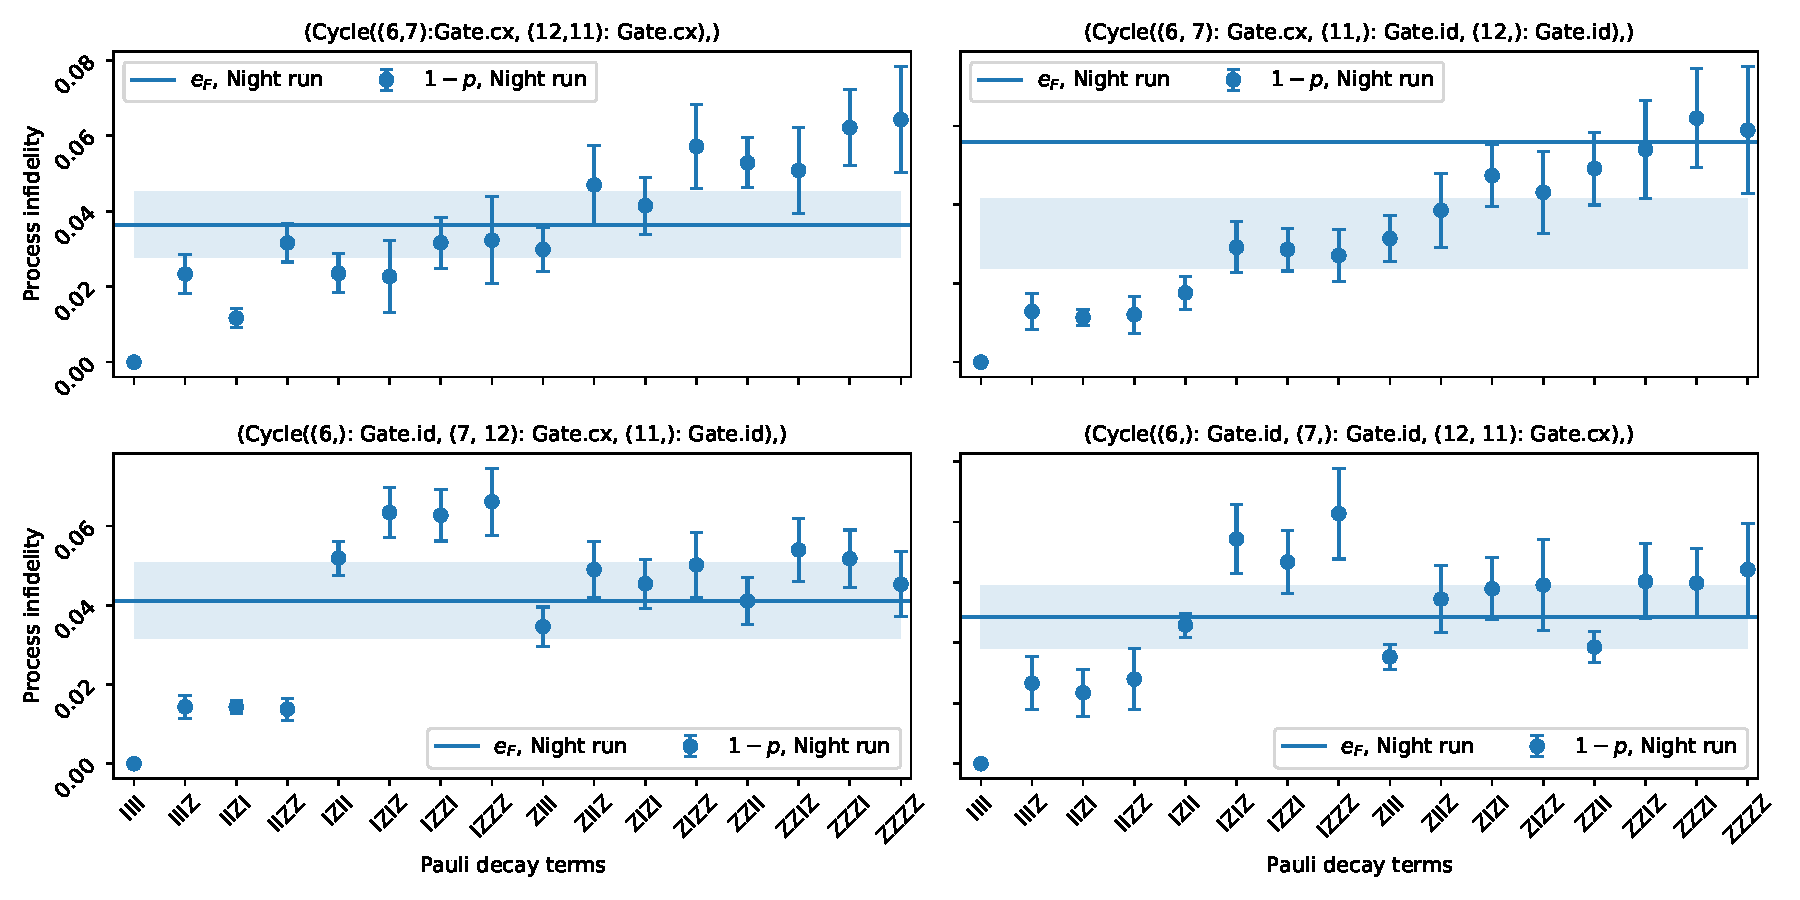
\includegraphics[scale=0.56]{CBPauliInfidelities_30_01_2021_NightRun_Layout2_Cycle1_2_3_4.pdf}
    \caption{The Pauli infidelities for each hard cycle calculated for each Pauli decay term from night run of layout 2 (qubits [6, 7, 12, 11]) on day 01/30/2021. The shaded regions show the error on the process infidelity and the error bars on the markers show the statistical errors on Pauli decay terms. }
    \label{fig:PauliInfidelities30Night_Story7}
\end{figure*}



\begin{figure}[htpb]
    % \centering
    % \includegraphics[width=2.2\columnwidth]{final_plot.pdf}
    % 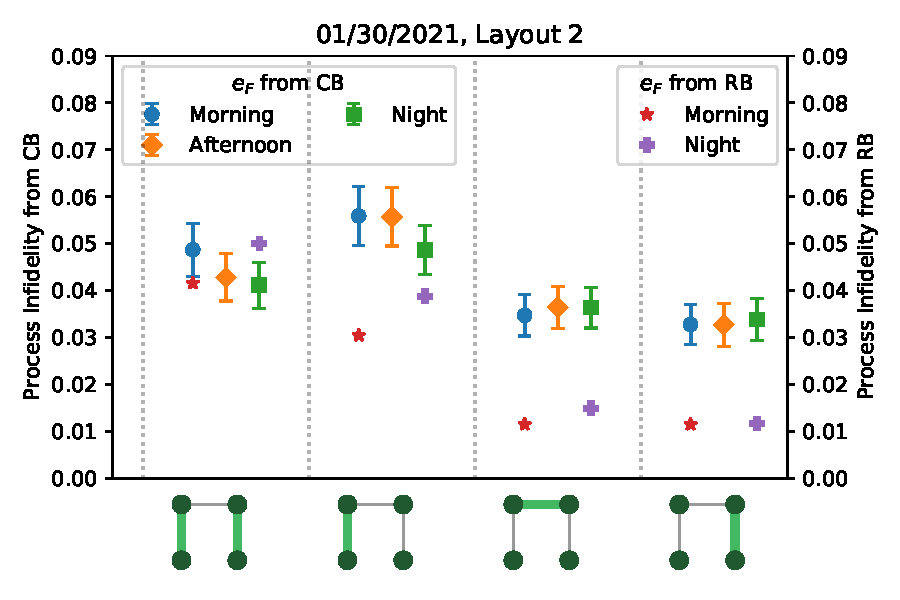
\includegraphics[scale=0.5]{ProcessInfidelities_CB_RB_Data_01_30_2021Layout2aligned.pdf}
    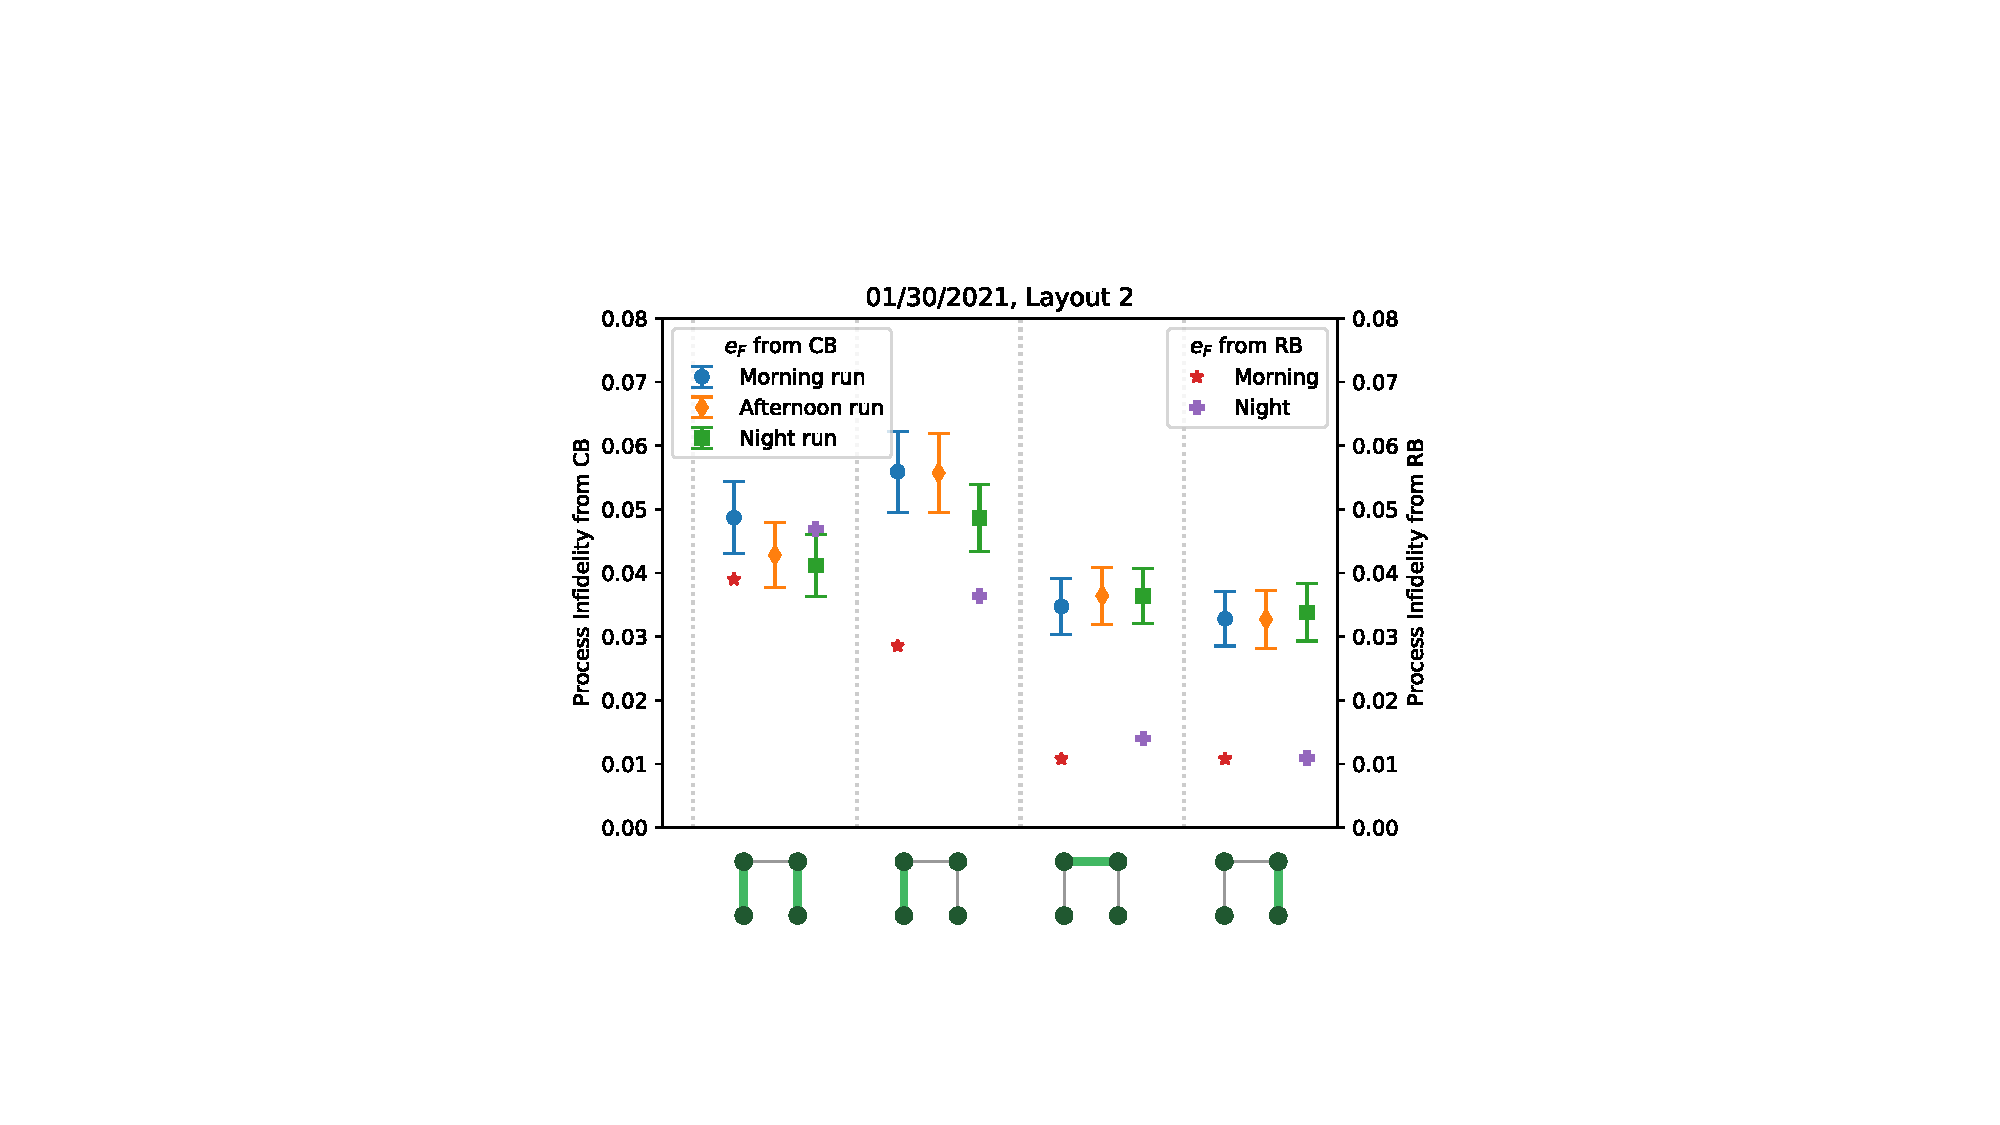
\includegraphics[scale=0.5]{ProcessInfidelitiesCB_RB_plots_30_morning_afternoon_night_L2.pdf}
    \caption{The process infidelities for cycles  1, 2, 3, and 4 calculated using randomized benchmarking (RB) (right axis) and cycle benchmarking (CB) (left axis) from morning, night, and afternoon runs of layout 2 (qubits [6, 7, 12, 11]) on days 01/30/2021.}
    \label{fig:processinfidelitiesStory7}
\end{figure}


\begin{figure}[htpb]
    % \centering
    % \includegraphics[width=2.2\columnwidth]{final_plot.pdf}
    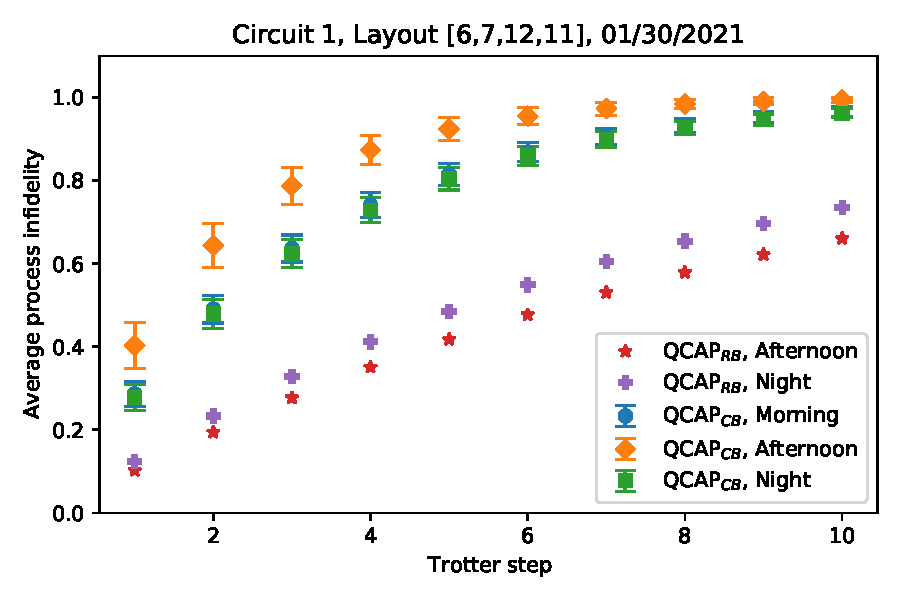
\includegraphics[scale=0.56]{QCAP_CB_RB_Data_01_30_2021_Layout_2C1.pdf}
    \caption{The QCAP bound as a function of number Trotter steps calculated using randomized benchmarking (QCAP$_{\text{RB}}$) (right axis) and cycle benchmarking (QCAP$_{\text{CB}}$) (left axis) from morning and afternoon runs of layout 2 (qubits [6, 7, 12, 11]) on days 01/30/2021.}
    \label{fig:QCAPCB_RB_Story7}
\end{figure}

\begin{figure}[htpb]
    % \centering
    % \includegraphics[width=2.2\columnwidth]{final_plot.pdf}
    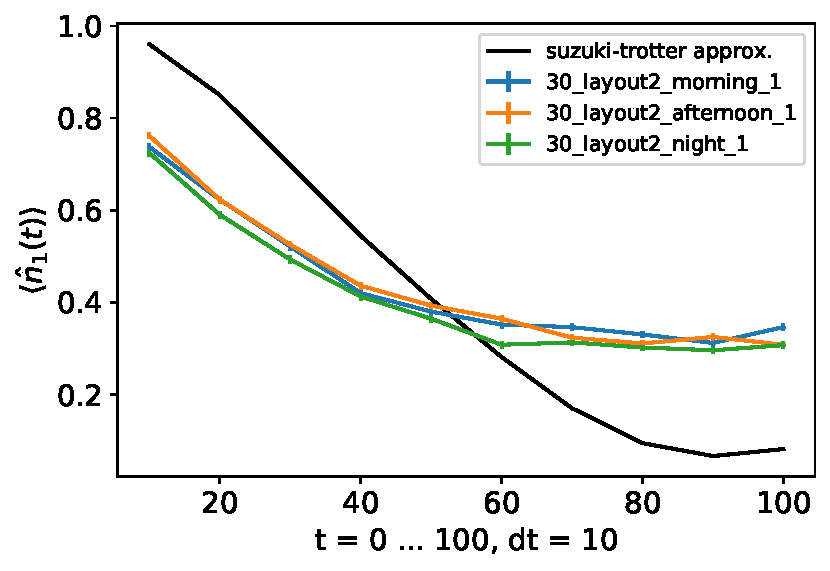
\includegraphics[scale=0.55]{TIM_[30]_[layout2]_[morning, afternoon, night]_n1.pdf}
    \caption{The particle number in site 1 calculated as a function of time from morning, afternoon and night runs on layout 2 (qubits [6, 7, 12, 11]) on day 01/30/2021 compared to exact Suzuki-Trotter approximation.}
    \label{fig:n1_Story7}
\end{figure}

Finally, using cycle benchmarking for the entire circuit 1 the QCAP bound as a function of number Trotter steps was calculated and compared to the randomized benchmarking data taken from the IBM back end properties for January 30, 2021 (Fig.~\ref{fig:QCAPCB_RB_Story7}).


%======================================================================================================
%======================================================================================================
%======================================================================================================

\subsection{Concurrent Computation Inconsistency Using Different QC Hardware Platform Qubits}
\label{sec:concurrent-computation-inconsistency-analysis}


Some researchers have recently put forward the idea of making duplicate copies of their quantum circuit and physically locating them on qubits in different areas of the processor for larger size quantum computing hardware platforms.  This technique in effect tries to parallelize the computation so that additional data and better statistics for the quantum circuit can be obtained more rapidly.

Our group ran experiments with this technique using cycle benchmarking and selecting a specific date and time to load identical copies of circuit 1 onto qubits located in different physical areas of the hardware platform.  The objective of these measurements was to indeed verify that the quantum hardware platform indeed produced a consistent set of results within error bars when comparing the outputs of circuit 1 run on these two physically separated sets of qubits.

In this section we report on the results of this technique.  We selected circuit 1 for the cycle benchmarking computations and ran this circuit on layout 1 and layout 2 after the IBM night calibration of Boeblingen on January 25th and again after the morning calibrations on January 27th. Figure~\ref{fig:QCAP_CB_RB_Data_01_25_2021_Layout_1_2C1_Night} shows both a graph of the cycle benchmarking average process infidelity versus Trotter step for circuit 1 run on both Layout 1 and 2 and a graph of the measurements from the random benchmarking calibration of Boeblingen by the IBM team after the night calibration on January 25th.  Figure~\ref{fig:QCAP_CB_RB_Data_01_27_2021_Layout_1_2C1_Morning} shows a similar plot for circuit 1 implemented on layout 1 and 2 and a graph of the measurements from the random benchmarking calibration of Boeblingen by the IBM team after the night calibration on January 27th.

What is clear from both graphs is that identical copies of circuit 1 executed on the Boeblingen processor on the same date and time but implemented on different groups of qubits physically separated on the processor produced sufficiently different values of the QCAP bounds that these values were beyond the overlaps of any of their combined error bars from each of the calculations.  Essentially these graphs are indicating that the results from the same calculation implemented in parallel on different physically displaced sets of qubits have only a limited capability to deliver consistent results.

%%%%%%



% Please add the following required packages to your document preamble:
% \usepackage{multirow}
% \usepackage[table,xcdraw]{xcolor}
% If you use beamer only pass "xcolor=table" option, i.e. \documentclass[xcolor=table]{beamer}
\begin{table*}[]
\begin{tabular}{|
>{\columncolor[HTML]{FFFFFF}}c |c|c|c|c|c|c|}
\hline
\multicolumn{7}{|c|}{\cellcolor[HTML]{FFFFFF}{\color[HTML]{333333} \textbf{Circuit result Consistency Between Layout 1 and 2}}}                                                                                                                                                                                                                                                                                  \\ \hline
\textbf{}                                                                                                           & \textbf{Qubits} & \cellcolor[HTML]{FFFFFF}\textbf{T1} ($\mu s$) & \cellcolor[HTML]{FFFFFF}\textbf{T2} ($\mu s$) & \begin{tabular}[c]{@{}c@{}} Readout \\ Error\\ $10^{-2}$ \end{tabular} & \begin{tabular}[c]{@{}c@{}} U2 \\ $10^{-4}$  \end{tabular} & \begin{tabular}[c]{@{}c@{}} U3\\ $10^{-4}$ \end{tabular} \\ \hline
\cellcolor[HTML]{FFFFFF}                                                                                            & 0               & \cellcolor[HTML]{FFFFFF}102.35      & \cellcolor[HTML]{FFFFFF}168.64      & 3.02                                                          & 2.87                                               & 5.74                                               \\ \cline{2-7} 
\cellcolor[HTML]{FFFFFF}                                                                                            & 1               & \cellcolor[HTML]{FFFFFF}41.62       & \cellcolor[HTML]{FFFFFF}74.29       & 11.44                                                         & 3.05                                               & 6.71                                               \\ \cline{2-7} 
\cellcolor[HTML]{FFFFFF}                                                                                            & 2               & \cellcolor[HTML]{FFFFFF}100.07      & \cellcolor[HTML]{FFFFFF}132.43      & 5.19                                                          & 2.91                                               & 5.82                                               \\ \cline{2-7} 
\multirow{-4}{*}{\cellcolor[HTML]{FFFFFF}\begin{tabular}[c]{@{}c@{}}01/25/2021\\ Layout 1\\ Night Run\end{tabular}} & 3               & 114.09                              & 44.72                               & 2.55                                                          & 4.44                                               & 8.88                                               \\ \hline
\cellcolor[HTML]{FFFFFF}                                                                                            & 6               & \cellcolor[HTML]{FFFFFF}70.46       & \cellcolor[HTML]{FFFFFF}109.1       & 2.09                                                          & 2.50                                               & 5.00                                               \\ \cline{2-7} 
\cellcolor[HTML]{FFFFFF}                                                                                            & 7               & \cellcolor[HTML]{FFFFFF}86.36       & \cellcolor[HTML]{FFFFFF}88.24       & 3.42                                                          & 3.97                                               & 7.94                                               \\ \cline{2-7} 
\cellcolor[HTML]{FFFFFF}                                                                                            & 12              & \cellcolor[HTML]{FFFFFF}63.41       & \cellcolor[HTML]{FFFFFF}88.23       & 3.76                                                          & 3.49                                               & 6.98                                               \\ \cline{2-7} 
\multirow{-4}{*}{\cellcolor[HTML]{FFFFFF}\begin{tabular}[c]{@{}c@{}}01/25/2021\\ Layout 2\\ Night Run\end{tabular}} & 11              & 82.69                               & 72.81                               & 4.68                                                          & 4.64                                               & 9.29                                               \\ \hline
\end{tabular}
\caption{test}
\end{table*}

% Please add the following required packages to your document preamble:
% \usepackage{multirow}
% \usepackage[table,xcdraw]{xcolor}
% If you use beamer only pass "xcolor=table" option, i.e. \documentclass[xcolor=table]{beamer}
\begin{table*}[]
\begin{tabular}{|
>{\columncolor[HTML]{FFFFFF}}c |c|c|c|c|c|c|}
\hline
\multicolumn{7}{|c|}{\cellcolor[HTML]{FFFFFF}{\color[HTML]{333333} \textbf{Consistency Across Circuit 1}}}                                                                                                                                                                                                                                                                                                                                                                                        \\ \hline
\textbf{}                                                                                                             & \textbf{Qubits} & \cellcolor[HTML]{FFFFFF}\textbf{\begin{tabular}[c]{@{}c@{}}T1\\ ($\mu$s )\end{tabular}} & \cellcolor[HTML]{FFFFFF}\textbf{\begin{tabular}[c]{@{}c@{}}T2\\ ($\mu$s)\end{tabular}} & \begin{tabular}[c]{@{}c@{}}Readout Error\\ $10^{-2}$ \end{tabular} & \begin{tabular}[c]{@{}c@{}}U2\\ $10^{-4}$ \end{tabular} & \begin{tabular}[c]{@{}c@{}}U3\\ $10^{-4}$ \end{tabular} \\ \hline
\cellcolor[HTML]{FFFFFF}                                                                                              & 0               & \cellcolor[HTML]{FFFFFF}63.09                                                         & \cellcolor[HTML]{FFFFFF}109.5                                                         & 6.57                                                          & 24.45                                              & 48.84                                              \\ \cline{2-7} 
\cellcolor[HTML]{FFFFFF}                                                                                              & 1               & \cellcolor[HTML]{FFFFFF}79.81                                                         & \cellcolor[HTML]{FFFFFF}96.80                                                         & 2.29                                                          & 3.79                                              & 7.57                                              \\ \cline{2-7} 
\cellcolor[HTML]{FFFFFF}                                                                                              & 2               & \cellcolor[HTML]{FFFFFF}87.31                                                         & \cellcolor[HTML]{FFFFFF}95.30                                                         & 5.15                                                          & 3.18                                              & 6.35                                              \\ \cline{2-7} 
\multirow{-4}{*}{\cellcolor[HTML]{FFFFFF}\begin{tabular}[c]{@{}c@{}}01/27/2021\\ Layout 1\\ Morning Run\end{tabular}} & 3               & 80.12                                                                                 & 36.64                                                                                 & 3.57                                                          & 3.46                                              & 6.91                                              \\ \hline
\cellcolor[HTML]{FFFFFF}                                                                                              & 6               & \cellcolor[HTML]{FFFFFF}24.11                                                         & \cellcolor[HTML]{FFFFFF}8.38                                                         & 2.56                                                          & 18.48                                              & 36.92                                              \\ \cline{2-7} 
\cellcolor[HTML]{FFFFFF}                                                                                              & 7               & \cellcolor[HTML]{FFFFFF}55.44                                                         & \cellcolor[HTML]{FFFFFF}103.00                                                      & 2.56                                                          & 3.43                                              & 6.89                                              \\ \cline{2-7} 
\cellcolor[HTML]{FFFFFF}                                                                                              & 12              & \cellcolor[HTML]{FFFFFF}102.00                                                      & \cellcolor[HTML]{FFFFFF}73.98                                                         & 4.49                                                          & 2.95                                              & 5.90                                              \\ \cline{2-7} 
\multirow{-4}{*}{\cellcolor[HTML]{FFFFFF}\begin{tabular}[c]{@{}c@{}}01/27/2021\\ Layout 2\\ Morning Run\end{tabular}} & 11              & 91.07                                                                                 & 116.4                                                                                 & 3.52                                                          & 4.64                                              & 9.28                                              \\ \hline
\end{tabular}
\end{table*}







%%%%%%%%


\begin{table}[]
\begin{tabular}{|
>{\columncolor[HTML]{FFFFFF}}c |
>{\columncolor[HTML]{FFFFFF}}c |
>{\columncolor[HTML]{FFFFFF}}c |
>{\columncolor[HTML]{FFFFFF}}c |}
\hline
\multicolumn{4}{|c|}{\cellcolor[HTML]{FFFFFF}{\color[HTML]{333333} \textbf{Layout 2 Intra-Day Two-Qubit Gate Error}}}                                                                                               \\ \hline
\textbf{}                                                                                                  & \textbf{Cycle} & \textbf{Qubits} & \textbf{\begin{tabular}[c]{@{}c@{}}CNOT Error\\ $10^{-2}$\end{tabular}} \\ \hline
\cellcolor[HTML]{FFFFFF}                                                                                   & 2              & [6,7]           & 3.226                                                               \\ \cline{2-4} 
\cellcolor[HTML]{FFFFFF}                                                                                   & 3              & [7,12]          & 1.078                                                               \\ \cline{2-4} 
\multirow{-3}{*}{\cellcolor[HTML]{FFFFFF}\begin{tabular}[c]{@{}c@{}}01/27/2021\\ Morning Run\end{tabular}} & 4              & [12,11]         & 0.9712                                                              \\ \hline
\cellcolor[HTML]{FFFFFF}                                                                                   & 2              & [6,7]           & 3.375                                                               \\ \cline{2-4} 
\cellcolor[HTML]{FFFFFF}                                                                                   & 3              & [7,12]          & 1.116                                                               \\ \cline{2-4} 
\multirow{-3}{*}{\cellcolor[HTML]{FFFFFF}\begin{tabular}[c]{@{}c@{}}01/27/2021\\ Night Run\end{tabular}}   & 4              & [12,11]         & 1.128                                                               \\ \hline
\cellcolor[HTML]{FFFFFF}                                                                                   & 2              & [6,7]           & 2.853                                                               \\ \cline{2-4} 
\cellcolor[HTML]{FFFFFF}                                                                                   & 3              & [7,12]          & 1.078                                                               \\ \cline{2-4} 
\multirow{-3}{*}{\cellcolor[HTML]{FFFFFF}\begin{tabular}[c]{@{}c@{}}01/30/2021\\ Morning Run\end{tabular}} & 4              & [12,11]         & 1.078                                                               \\ \hline
\cellcolor[HTML]{FFFFFF}                                                                                   & 2              & [6,7]           & 3.638                                                               \\ \cline{2-4} 
\cellcolor[HTML]{FFFFFF}                                                                                   & 3              & [7,12]          & 1.398                                                               \\ \cline{2-4} 
\multirow{-3}{*}{\cellcolor[HTML]{FFFFFF}\begin{tabular}[c]{@{}c@{}}01/30/2021\\ Night Run\end{tabular}}   & 4              & [12,11]         & 1.093                                                               \\ \hline
\end{tabular}
\end{table}












\begin{figure}[htpb]
    % \centering
    % \includegraphics[width=2.2\columnwidth]{final_plot.pdf}
    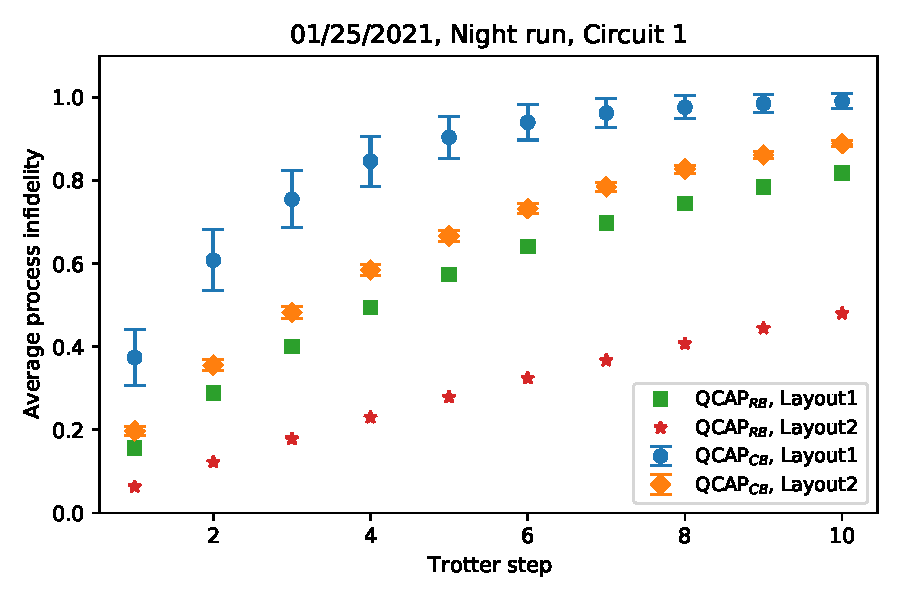
\includegraphics[scale=0.56]{QCAP_CB_RB_Data_01_25_2021_Layout_1_2C1_Night.pdf}
    \caption{The QCAP bound as a function of number Trotter steps calculated using randomized benchmarking (QCAP$_{\text{RB}}$) (right axis) and cycle benchmarking (QCAP$_{\text{CB}}$) (left axis) from the night run of circuit 1 on both layout 1 (qubits [0, 1, 2, 3]) and layout 2 (qubits [6, 7, 12, 11]) on January 25, 2021.}
    \label{fig:QCAP_CB_RB_Data_01_25_2021_Layout_1_2C1_Night}
\end{figure}


\begin{figure}[htpb]
    % \centering
    % \includegraphics[width=2.2\columnwidth]{final_plot.pdf}
    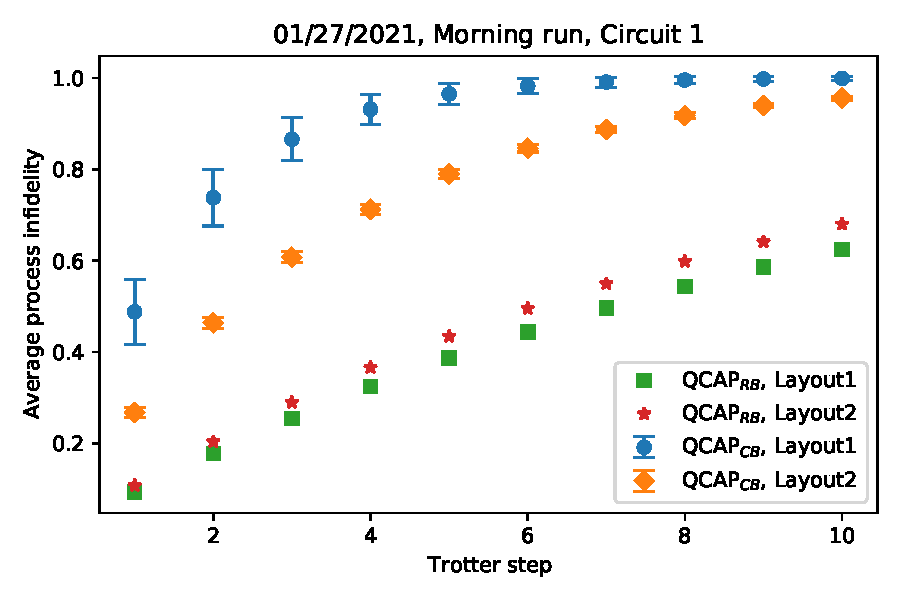
\includegraphics[scale=0.56]{QCAP_CB_RB_Data_01_27_2021_Layout_1_2C1_Morning.pdf}
    \caption{The QCAP bound as a function of number Trotter steps calculated using randomized benchmarking (QCAP$_{\text{RB}}$) (right axis) and cycle benchmarking (QCAP$_{\text{CB}}$) (left axis) from the morning run of circuit 1 on both layout 1 (qubits [0, 1, 2, 3]) and layout 2 (qubits [6, 7, 12, 11]) on January 27, 2021.}
    \label{fig:QCAP_CB_RB_Data_01_27_2021_Layout_1_2C1_Morning}
\end{figure}
















The process infidelity of each cycle obtained using cycle benchmarking and randomized benchmarking for night run on Layout 2 (qubits [6, 7, 12, 11]) on day 01/25/2021 can be seen in Fig.~\ref{fig:processinfidelitiesStory5}.

\begin{figure}[htpb]
    % \centering
    % \includegraphics[width=2.2\columnwidth]{final_plot.pdf}
    % 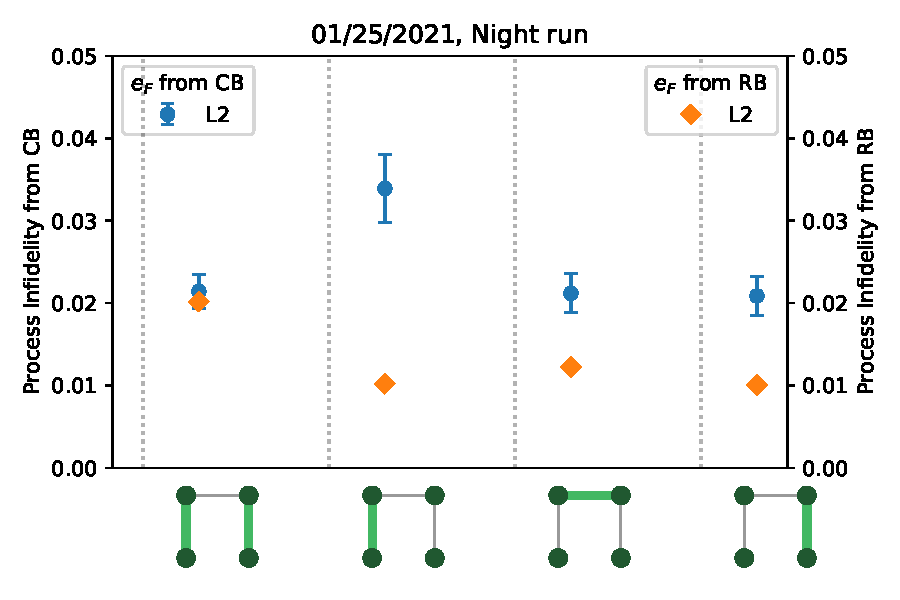
\includegraphics[scale=0.5]{ProcessInfidelities_CB_RB_Data_01_25_2021Layout2aligned.pdf}
    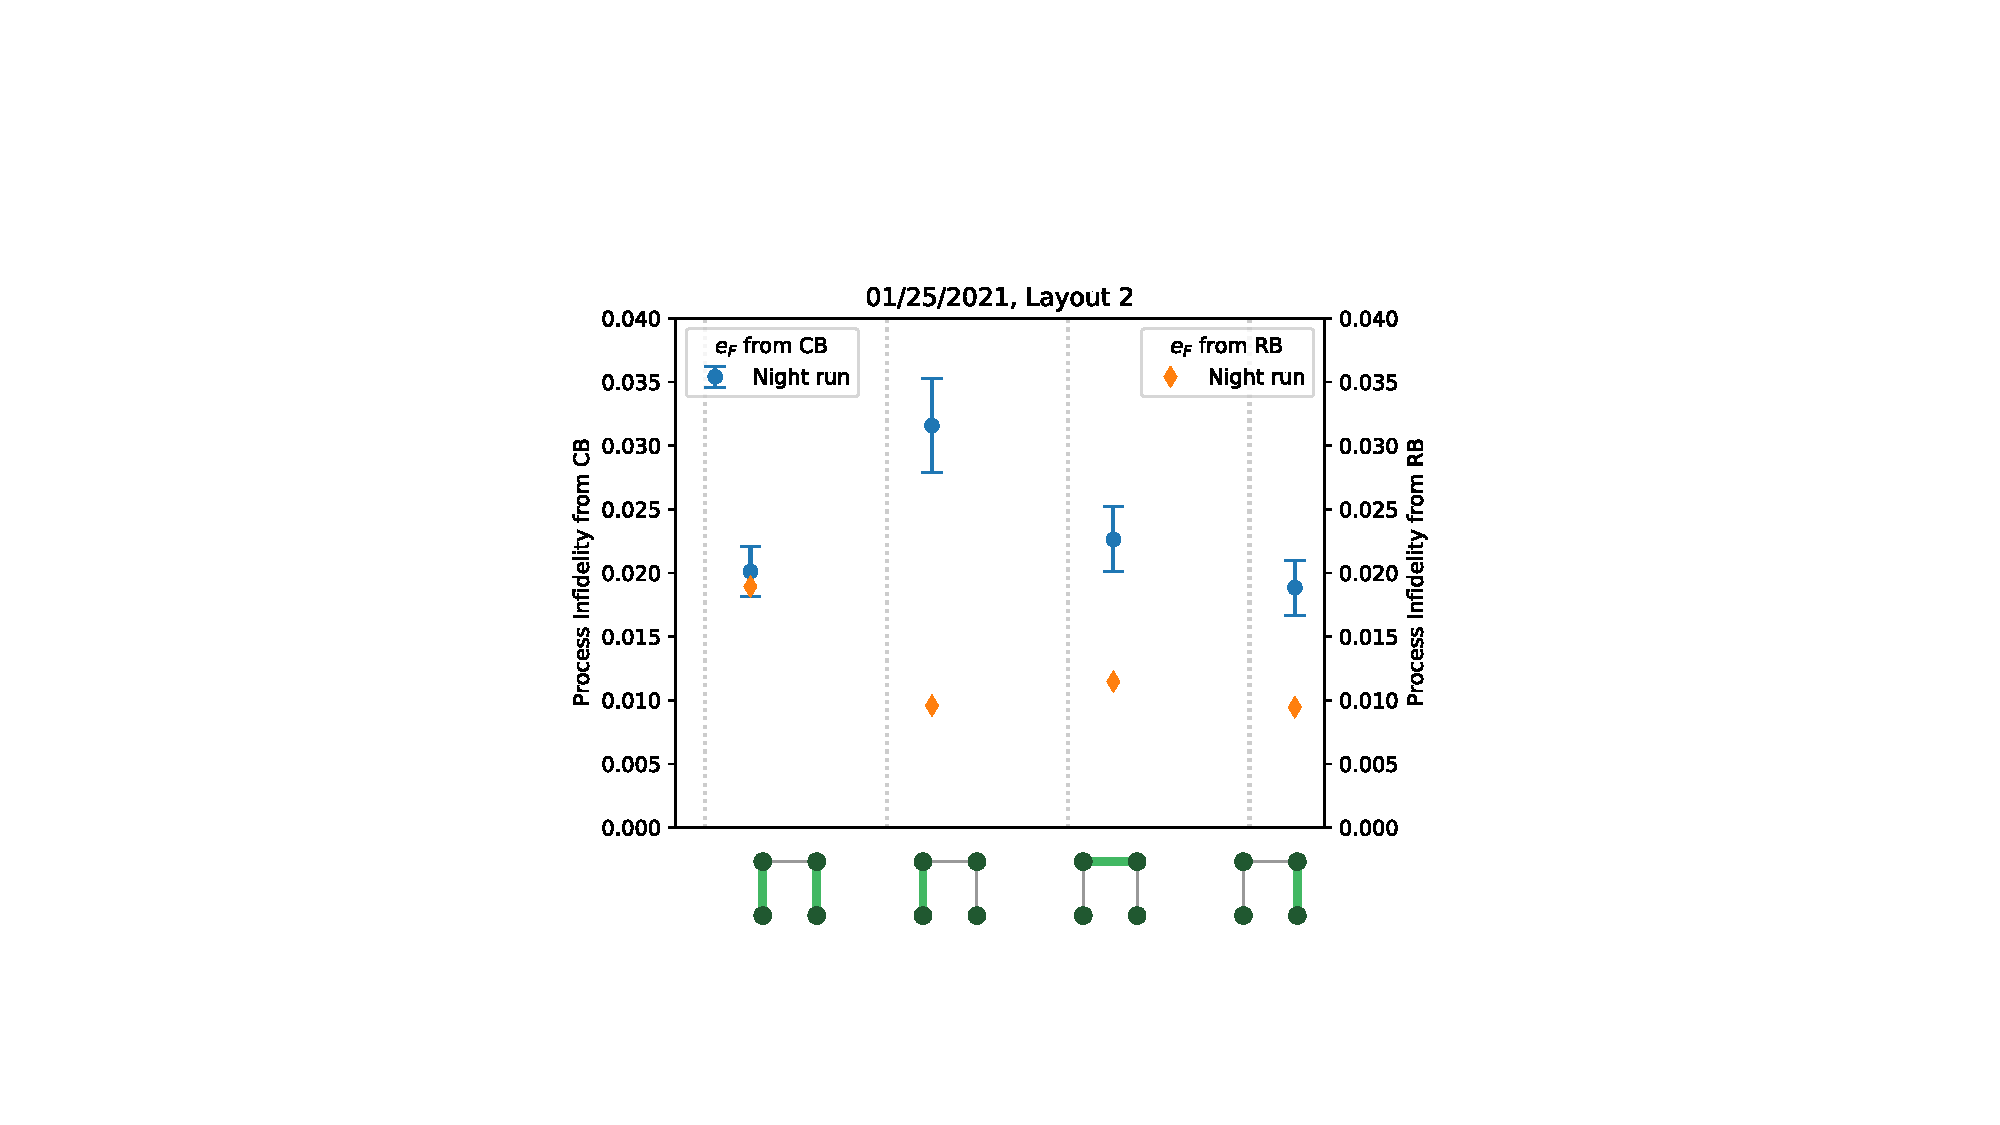
\includegraphics[scale=0.5]{ProcessInfidelitiesCB_RB_plots_25_night_L2.pdf}
    \caption{The process infidelities for cycles  1, 2, 3, and 4 calculated using randomized benchmarking (RB) (right axis) and cycle benchmarking (CB) (left axis) from night run of layout 2 (qubits [6, 7, 12, 11]) on day 01/25/2021.}
    \label{fig:processinfidelitiesStory5}
\end{figure}

The QCAP$_{\text{CB}}$ and QCAP$_{\text{RB}}$ values as a function of number Trotter steps for night run on layout 2 (qubits [6, 7, 12, 11]) on day 01/25/2021 can be seen in Fig.~\ref{fig:QCAPCB_RB_Story5}.

\begin{figure}[htpb]
    % \centering
    % \includegraphics[width=2.2\columnwidth]{final_plot.pdf}
    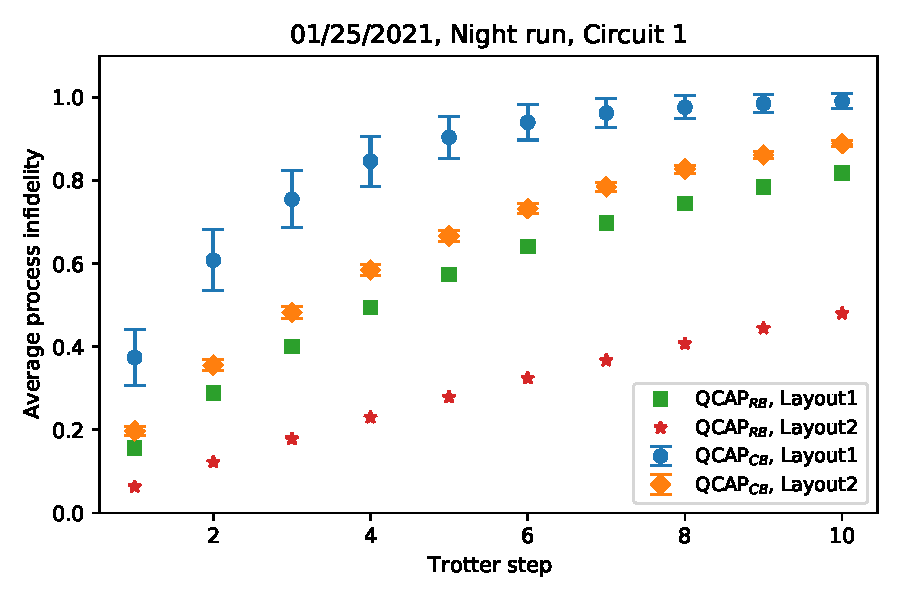
\includegraphics[scale=0.56]{QCAP_CB_RB_Data_01_25_2021_Layout_1_2C1_Night.pdf}
    \caption{The QCAP bound as a function of number Trotter steps calculated using randomized benchmarking (QCAP$_{\text{RB}}$) (right axis) and cycle benchmarking (QCAP$_{\text{CB}}$) (left axis) from night run of layout 2 (qubits [6, 7, 12, 11]) on day 01/25/2021.}
    \label{fig:QCAPCB_RB_Story5}
\end{figure}

The particle number in site 1 as a function of time comparing exact Trotter values with the values obtained from night run on layout 1 (qubits [0,1,2,3]) and 2 (qubits [6, 7, 12, 11]) on day 01/25/2021 can be seen in Fig.~\ref{fig:n1_Story5}.

\begin{figure}[htpb]
    % \centering
    % \includegraphics[width=2.2\columnwidth]{final_plot.pdf}
    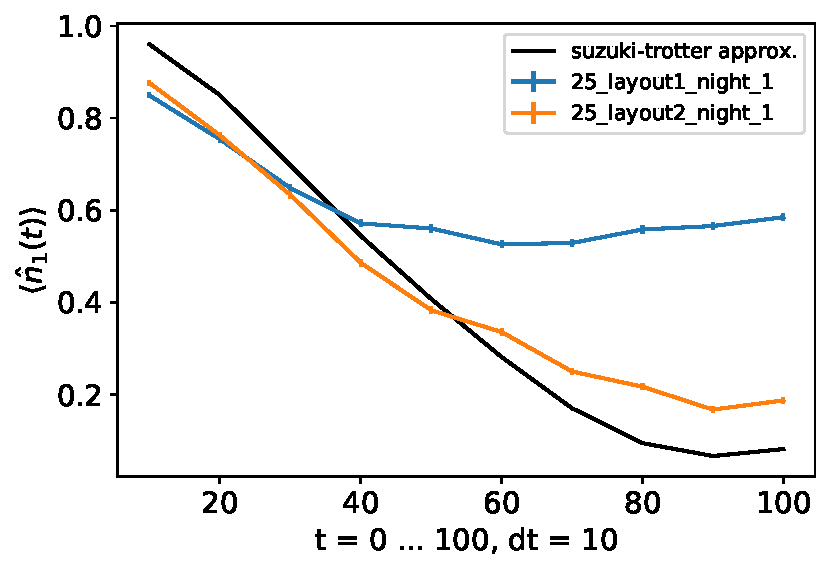
\includegraphics[scale=0.55]{TIM_[25]_[layout1, layout2]_[night]_n1.pdf}
    \caption{The particle number in site 1 calculated as a function of time from night run on layout 1 (qubits [0, 1, 2, 3]) and layout 2 (qubits [6, 7, 12, 11]) on day 01/25/2021 compared to exact Suzuki-Trotter approximation.}
    \label{fig:n1_Story5}
\end{figure}

\begin{figure*}[htpb]
    % \centering
    % \includegraphics[width=2.2\columnwidth]{final_plot.pdf}
    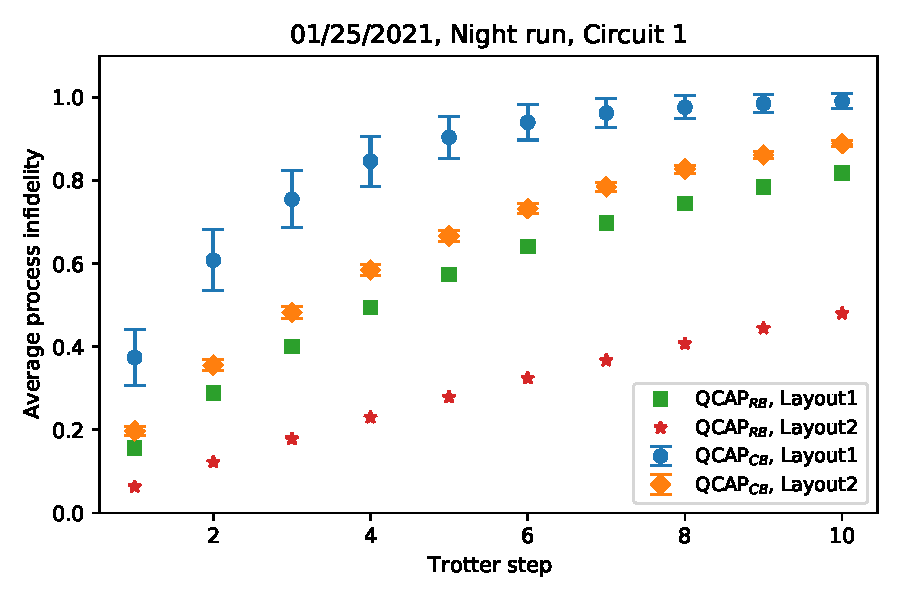
\includegraphics[scale=0.55]{QCAP_CB_RB_Data_01_25_2021_Layout_1_2C1_Night.pdf}
    \includegraphics[scale=0.55]{QCAP_CB_RB_Data_01_25_2021_Layout_1_2C2_Night.pdf}
    \caption{The QCAP bound as a function of number Trotter steps calculated using randomized benchmarking (QCAP$_{\text{RB}}$) and cycle  benchmarking (QCAP$_{\text{CB}}$) from night run of layout 1 and 2 on day 01/25/2021 for Circuit 1 (left panel) and Circuit 2 (right panel) with only CNOT gates used as hard cycles. The  plotted  error  bars  only show the statistical error.}
    \label{fig:QCAP_circ1_circ2_25th_L1L2_Night}
\end{figure*}





\subsection{QCAP Bound Performance of Different Gate Combinations Giving the Same Physics}
\label{sec:circ1_vs_circ2_QCAP}

In this section, we discuss the QCAP bound performance of the two quantum circuits as seen in Fig.~\ref{fig:IsingTrotterCircs} with different gate layout for TIM Trotter step that gives the same physics. As discussed above, in our QCAP calculations we used CNOT gates as our hard gates since two-qubit errors are the dominant source of error in the quantum circuit. Therefore, we can say that the QCAP bound values that we calculated are lower bound to the exact error due to errors in single and two-qubit gates in the quantum circuit. The hard cycles used at each Trotter step for circuit 1 and circuit 2 can be seen in Fig.~\ref{fig:hardcycles}.  
% \begin{figure}[htpb]
%     % \centering
%     % \includegraphics[width=2.2\columnwidth]{final_plot.pdf}
%     \includegraphics[scale=0.50]{hardcyclesCirc1Circ2.pdf}
%     \caption{The CNOT hard cycles used at each Trotter step for circuit 1 ({\bf{(a)}}) and circuit 2 ({\bf{(b)}}) to calculate QCAP$_{\text{CB}}$ bound from cycle benchmarking are shown in dashed boxes.}
%     \label{fig:hardcycles}
% \end{figure}

% \begin{figure*}[ht!]
%     % \centering
%     % \includegraphics[width=2.2\columnwidth]{final_plot.pdf}
%     \includegraphics[scale=0.55]{QCAP_CB_RB_Data_01_24_2021_Layout_2C1_C2_Morning.pdf}
%     \includegraphics[scale=0.55]{QCAP_CB_RB_Data_01_29_2021_Layout_2C1_C2_Morning.pdf}
%     \caption{The QCAP bound as a function of number Trotter steps calculated using randomized benchmarking (QCAP$_{\text{RB}}$) and cycle  benchmarking (QCAP$_{\text{CB}}$) from morning run of layout 2 (qubits [6, 7, 12, 11]) on days 01/24/2021 (left panel) and 01/29/2021 (right panel) for Circuit 1 and Circuit 2 with only CNOT gates used as hard cycles. The  plotted  error  bars  only show the statistical error.}
%     \label{fig:QCAP_circ1_circ2_24th_29th_L2_Morning}
% \end{figure*}

% \begin{figure}[ht!]
%     % \centering
%     \includegraphics[scale=0.55]{QCAP_CB_RB_Data_01_25_2021_Layout_2C1_C2_Morning.pdf}
%     \caption{The QCAP bound as a function of number Trotter steps calculated using randomized benchmarking (QCAP$_{\text{RB}}$) and cycle  benchmarking (QCAP$_{\text{CB}}$) from morning run of layout 2 on day 01/25/2021 for Circuit 1 and Circuit 2 with only CNOT gates used as hard cycles. The  plotted  error  bars  only show the statistical error.}
%     \label{fig:QCAP_circ1_circ2_25th_L2_Morning}
% \end{figure}

\begin{figure*}[htpb]
    % \centering
    % \includegraphics[width=2.2\columnwidth]{final_plot.pdf}
    \includegraphics[scale=0.36]{QCAP_CB_RB_Data_01_24_2021_Layout_2C1_C2_Morning.pdf}
    \includegraphics[scale=0.36]{QCAP_CB_RB_Data_01_25_2021_Layout_2C1_C2_Morning.pdf}
    \includegraphics[scale=0.36]{QCAP_CB_RB_Data_01_29_2021_Layout_2C1_C2_Morning.pdf}
    \caption{The QCAP bound as a function of number Trotter steps calculated using randomized benchmarking (QCAP$_{\text{RB}}$) and cycle  benchmarking (QCAP$_{\text{CB}}$) from morning run of layout 2 (qubits [6, 7, 12, 11]) on days 01/24/2021 (left panel), 01/25/2021 (middle panel) and 01/29/2021 (right panel) for Circuit 1 and Circuit 2 with only CNOT gates used as hard cycles. The  plotted  error  bars  only show the statistical error.}
    \label{fig:QCAP_circ1_circ2_24th_25th_29th_L2_Morning}
\end{figure*}
In Fig.~\ref{fig:QCAP_circ1_circ2_24th_25th_29th_L2_Morning} we demonstrate the QCAP$_{\text{CB}}$ bound for the CNOT hard cycles in circuit 1 and circuit 2 (Fig.~\ref{fig:hardcycles}) as a function of Trotter steps for morning run on layout 2 (qubits [6,7,11,12]) on days 01/24-25-29/2021, respectively. These figures show that the QCAP$_{\text{CB}}$ bound for circuit 2 is higher than the QCAP$_{\text{CB}}$ bound for circuit 1. This is an expected result as the quantum circuit depth for circuit 2 is greater than the circuit depth for circuit 1. However, these results are interesting since they show how fast the QCAP$_{\text{CB}}$ bound can grow when the order of gates is not done wisely. On the other hand, since individual CNOT gates are used when the process infidelity is calculated from randomized benchmarking the QCAP$_{\text{RB}}$ bound calculated from \eqref{eq:QCAP_RB} does not depend on the CNOT layout in the circuit, i.e. it only depends on the number of CNOT gates in the circuit. Therefore, it does not reflect how fast the errors can grow in the quantum circuit depending on the circuit depth.